%===============================================================================
% LaTeX sjabloon voor de bachelorproef toegepaste informatica aan HOGENT
% Meer info op https://github.com/HoGentTIN/latex-hogent-report
%===============================================================================

\documentclass[dutch,dit,thesis]{hogentreport}

% TODO:
% - If necessary, replace the option `dit`' with your own department!
%   Valid entries are dbo, dbt, dgz, dit, dlo, dog, dsa, soa
% - If you write your thesis in English (remark: only possible after getting
%   explicit approval!), remove the option "dutch," or replace with "english".

\usepackage{lipsum} % For blind text, can be removed after adding actual content
\usepackage{fontspec}
\setmonofont{Courier New} % Replace with a font that is installed on your system
%% Pictures to include in the text can be put in the graphics/ folder
\graphicspath{{../graphics/}}

%% For source code highlighting, requires pygments to be installed
%% Compile with the -shell-escape flag!
%% \usepackage[chapter]{minted}
%% If you compile with the make_thesis.{bat,sh} script, use the following
%% import instead:
\usepackage[chapter,outputdir=../output]{minted}
\usemintedstyle{solarized-light}

%% Formatting for minted environments.
\setminted{%
    autogobble,
    frame=lines,
    breaklines,
    linenos,
    tabsize=4
}

%% Ensure the list of listings is in the table of contents
\renewcommand\listoflistingscaption{%
    \IfLanguageName{dutch}{Lijst van codefragmenten}{List of listings}
}
\renewcommand\listingscaption{%
    \IfLanguageName{dutch}{Codefragment}{Listing}
}
\renewcommand*\listoflistings{%
    \cleardoublepage\phantomsection\addcontentsline{toc}{chapter}{\listoflistingscaption}%
    \listof{listing}{\listoflistingscaption}%
}

% Other packages not already included can be imported here

%%---------- Document metadata -------------------------------------------------
% TODO: Replace this with your own information
\author{Ernstqwqwq Aarden}
\supervisor{Dhr. F. Van Houte}
\cosupervisor{Mevr. S. Beeckman}
\title[Optionele ondertitel]%
    {Titel van de bachelorproef}
\academicyear{\advance\year by -1 \the\year--\advance\year by 1 \the\year}
\examperiod{1}
\degreesought{\IfLanguageName{dutch}{Professionele bachelor in de toegepaste informatica}{Bachelor of applied computer science}}
\partialthesis{false} %% To display 'in partial fulfilment'
%\institution{Internshipcompany BVBA.}

%% Add global exceptions to the hyphenation here
\hyphenation{back-slash}

%% The bibliography (style and settings are  found in hogentthesis.cls)
\addbibresource{bachproef.bib}            %% Bibliography file
\addbibresource{../voorstel/voorstel.bib} %% Bibliography research proposal
\defbibheading{bibempty}{}

%% Prevent empty pages for right-handed chapter starts in twoside mode
\renewcommand{\cleardoublepage}{\clearpage}

\renewcommand{\arraystretch}{1.2}

%% Content starts here.
\begin{document}

%---------- Front matter -------------------------------------------------------

\frontmatter

\hypersetup{pageanchor=false} %% Disable page numbering references
%% Render a Dutch outer title page if the main language is English
\IfLanguageName{english}{%
    %% If necessary, information can be changed here
    \degreesought{Professionele Bachelor toegepaste informatica}%
    \begin{otherlanguage}{dutch}%
       \maketitle%
    \end{otherlanguage}%
}{}

%% Generates title page content
\maketitle
\hypersetup{pageanchor=true}

%%=============================================================================
%% Voorwoord
%%=============================================================================

\chapter*{\IfLanguageName{dutch}{Woord vooraf}{Preface}}%
\label{ch:voorwoord}

%% TODO:
%% Het voorwoord is het enige deel van de bachelorproef waar je vanuit je
%% eigen standpunt (``ik-vorm'') mag schrijven. Je kan hier bv. motiveren
%% waarom jij het onderwerp wil bespreken.
%% Vergeet ook niet te bedanken wie je geholpen/gesteund/... heeft

Met trots en voldoening presenteer ik deze bachelorproef, het sluitstuk van mijn opleiding Toegepaste Informatica aan de HoGent. In het begin toen ik begon met zoeken naar een onderwerp had ik geen idee waar ik moest beginnen en  vond ik dit dus ook een grote uitdaging. Ik begon met het zoeken naar bepaalde interessante onderwerpen en toen kwam ik uiteindelijk op dit onderwerp. Ik heb sterke interesses in cybersecurity dus  wou ik dit implementeren in mijn bachelorproef. Daarbij ontwikkelde ik ook interesse in back-ups tijdens het opleidingsonderdeel Cybersecurity Advanced. Het schrijven van deze bachelorproef was niet alleen een uitdagend leerproces, maar ook een unieke kans om mijn interesse in systeembeheer en cybersecurity verder te verdiepen. Dit project heeft me niet alleen geholpen mijn technische kennis te versterken, maar ook om praktijkervaring op te doen binnen een professionele context.

Ik wil graag mijn dankbaarheid uitdrukken aan mijn co-promotor, Rémy Tetaert, voor zijn waardevolle begeleiding, expertise en tijd tijdens dit proces. Zijn inzichten, ondersteuning en begeleiding waren heel belangrijk voor mij. Daarnaast wil ik mijn promotor, Martijn Saelens, bedanken voor zijn constructieve feedback en kritische blik, die me steeds hebben geholpen om mijn werk te verbeteren. 

Tot slot wil ik ook mijn familie en vrienden bedanken voor hun geduld, steun en motivatie gedurende deze periode. Zonder hen zou dit niet mogelijk zijn geweest.


%%=============================================================================
%% Samenvatting
%%=============================================================================

% TODO: De "abstract" of samenvatting is een kernachtige (~ 1 blz. voor een
% thesis) synthese van het document.
%
% Een goede abstract biedt een kernachtig antwoord op volgende vragen:
%
% 1. Waarover gaat de bachelorproef?
% 2. Waarom heb je er over geschreven?
% 3. Hoe heb je het onderzoek uitgevoerd?
% 4. Wat waren de resultaten? Wat blijkt uit je onderzoek?
% 5. Wat betekenen je resultaten? Wat is de relevantie voor het werkveld?
%
% Daarom bestaat een abstract uit volgende componenten:
%
% - inleiding + kaderen thema
% - probleemstelling
% - (centrale) onderzoeksvraag
% - onderzoeksdoelstelling
% - methodologie
% - resultaten (beperk tot de belangrijkste, relevant voor de onderzoeksvraag)
% - conclusies, aanbevelingen, beperkingen
%
% LET OP! Een samenvatting is GEEN voorwoord!

%%---------- Nederlandse samenvatting -----------------------------------------
%




\chapter*{Samenvatting}
Dit onderzoek heeft als doel de back-upstrategie van Forvis Mazars te analyseren en optimaliseren, met een focus op het verbeteren van de bescherming tegen cyberdreigingen zoals ransomware-aanvallen. Het bedrijf maakt gebruik van Azure voor het beheren van zijn data en heeft momenteel een back-upstrategie die bestaat uit automatische full back-ups van twee databases en een manueel uitgevoerd script voor het maken van back-ups van specifieke databases naar een Azure Storage-account.

De bescherming van bedrijfsdata is essentieel voor het waarborgen van de continuïteit van een organisatie, en back-ups spelen hierbij een cruciale rol. Het oorspronkelijke back-upplan van Forvis Mazars was echter kwetsbaar omdat het geen gebruik maakte van immutable storage, waardoor de back-ups gevoelig waren voor manipulatie door aanvallers, bijvoorbeeld in het geval van ransomware.

Om de back-upstrategie te verbeteren, werd een Proof-of-Concept (PoC) ontwikkeld in een lokale testomgeving met VirtualBox, waarin de effectiviteit van immutable storage werd getest. In deze simulatie werd aangetoond dat immutable storage het mogelijk maakt om back-ups te beschermen tegen manipulatie, zelfs wanneer een aanvaller volledige controle heeft over het systeem. Dit werd bevestigd door het encrypten van back-upbestanden en het verwijderen van de actieve database, waarbij de integriteit van de immutabele back-ups behouden bleef.

Verder werd de huidige back-upstrategie van Forvis Mazars geanalyseerd, waarbij verschillende verbeterpunten werden geïdentificeerd. Aanbevelingen zoals het implementeren van immutable storage in de Azure-omgeving en het automatiseren van manuele back-ups via Kubernetes cronjobs werden geformuleerd. Deze verbeteringen dragen bij aan het vergroten van de veiligheid en betrouwbaarheid van de back-ups en zorgen voor snellere en effectievere herstelmogelijkheden.

In dit onderzoek werd ook een literatuurstudie uitgevoerd waarin verschillende back-upmethoden, technieken en ransomware-resistente oplossingen werden onderzocht. De opgedane kennis heeft bijgedragen aan het ontwikkelen van een geoptimaliseerde back-upstrategie voor Forvis Mazars, die niet alleen de veiligheid verhoogt, maar ook de bedrijfscontinuïteit beschermt tegen cyberaanvallen. De inzichten en technieken die in dit onderzoek zijn gepresenteerd, kunnen ook waardevolle toepassingen hebben voor andere organisaties die hun back-upstrategieën willen versterken, met name binnen Azure-omgevingen.

















%---------- Inhoud, lijst figuren, ... -----------------------------------------

\tableofcontents

% In a list of figures, the complete caption will be included. To prevent this,
% ALWAYS add a short description in the caption!
%
%  \caption[short description]{elaborate description}
%
% If you do, only the short description will be used in the list of figures

\listoffigures

% If you included tables and/or source code listings, uncomment the appropriate
% lines.
\listoftables

\listoflistings

% Als je een lijst van afkortingen of termen wil toevoegen, dan hoort die
% hier thuis. Gebruik bijvoorbeeld de ``glossaries'' package.
% https://www.overleaf.com/learn/latex/Glossaries

%---------- Kern ---------------------------------------------------------------

\mainmatter{}

% De eerste hoofdstukken van een bachelorproef zijn meestal een inleiding op
% het onderwerp, literatuurstudie en verantwoording methodologie.
% Aarzel niet om een meer beschrijvende titel aan deze hoofdstukken te geven of
% om bijvoorbeeld de inleiding en/of stand van zaken over meerdere hoofdstukken
% te verspreiden!

%%=============================================================================
%% Inleiding
%%=============================================================================

\chapter{\IfLanguageName{dutch}{Inleiding}{Introduction}}%
\label{ch:inleiding}

De beveiliging van gegevens is van cruciaal belang voor organisaties, vooral gezien de toenemende dreigingen van cyberaanvallen zoals ransomware. Gezien de digitale transformatie die veel bedrijven doormaken, zijn betrouwbare en veilige back-up oplossingen essentieel om de continuïteit van de bedrijfsvoering te waarborgen. Dit geldt in het bijzonder voor bedrijven die werken met cloudplatformen zoals Microsoft Azure, waar databases zoals PostgreSQL en MySQL vaak cruciaal zijn voor het dagelijks functioneren. Bij Forvis Mazars worden momenteel back-ups van Azure-databases gemaakt via een combinatie van automatische volledige back-ups en handmatige back-ups via scripts. Deze aanpak kent echter enkele beperkingen, zoals de onregelmatige uitvoering van de handmatige back-ups en een gebrek aan geautomatiseerde processen, wat de veiligheid en efficiëntie van het systeem in gevaar kan brengen.



\section{\IfLanguageName{dutch}{Probleemstelling}{Problem Statement}}%
\label{sec:probleemstelling}
In deze bachelorproef wordt de huidige back-upstrategie van Forvis Mazars geanalyseerd en geoptimaliseerd. De focus ligt hierbij op het verbeteren van de back-upstrategie voor de Azure PostgreSQL en MySQL databases, met bijzondere aandacht voor ransomware-resistentie en de integratie van immutabele opslagtechnieken. Het doel is om de bestaande strategie te versterken en de kans op dataverlies door cyberaanvallen te minimaliseren. Daarnaast zal er een proof-of-concept worden uitgevoerd om de effectiviteit van immutabele opslag te testen in een scenario waarbij een ransomware-aanval wordt nagebootst op mock-up bestanden. De probleemstelling van dit onderzoek is dat de huidige back-upstrategie bij Forvis Mazars niet voldoende robuust is om het risico op dataverlies door ransomware effectief te mitigeren. Dit onderzoek heeft tot doel de back-upstrategieën van Forvis Mazars te verbeteren door middel van geautomatiseerde processen en door gebruik te maken van immutabele opslag voor extra beveiliging tegen dataverlies. De doelgroep van dit onderzoek bestaat uit Forvis Mazars

\section{\IfLanguageName{dutch}{Onderzoeksvraag}{Research question}}%
\label{sec:onderzoeksvraag}

De onderzoeksvraag van deze bachelorproef luidt:

\textbf{Hoe kan de back-upstrategie voor Azure PostgreSQL en MySQL databases bij Forvis Mazars worden geoptimaliseerd met behulp van immutabele opslag en automatische back-ups?}

\section{Deelvragen}
De onderzoeksvraag kan verder opgedeeld worden in de volgende deelvragen.:
\begin{itemize}
    \item Hoe veilig en betrouwbaar zijn de huidige back-upoplossingen van Forvis Mazars voor Azure PostgreSQL en MySQL databases?
    \item Welke rol speelt immutabele opslag in het beschermen van back-ups tegen ransomware en andere vormen van dataverlies?
    \item Wat zijn de belangrijkste uitdagingen bij het integreren van immutabele opslag met Azure cloud back-upsystemen?
\end{itemize}

\section{\IfLanguageName{dutch}{Onderzoeksdoelstelling}{Research objective}}%
\label{sec:onderzoeksdoelstelling}

Het doel van dit onderzoek is om de back-upstrategie van Forvis Mazars te optimaliseren door de huidige back-upmethoden te analyseren en te verbeteren. Het onderzoek richt zich specifiek op het implementeren van immutabele opslag om de bescherming tegen ransomware-aanvallen te versterken. Daarnaast wordt de automatisering van de manuele back-ups onderzocht en geïmplementeerd, aangezien deze momenteel niet frequent genoeg worden uitgevoerd. Een proof-of-concept (PoC) zal worden uitgevoerd door virtuele machines te gebruiken en een ransomware-aanval na te bootsen om de effectiviteit van de immutabele opslag te testen. Dit proefproject zal verder bijdragen aan het verbeteren van de bestaande automatische back-upstructuur door het toevoegen van meer geautomatiseerde processen, wat de efficiëntie en de veiligheid van het back-upbeheer binnen het bedrijf zal vergroten.
\section{\IfLanguageName{dutch}{Opzet van deze bachelorproef}{Structure of this bachelor thesis}}%
\label{sec:opzet-bachelorproef}

% Het is gebruikelijk aan het einde van de inleiding een overzicht te
% geven van de opbouw van de rest van de tekst. Deze sectie bevat al een aanzet
% die je kan aanvullen/aanpassen in functie van je eigen tekst.

De rest van deze bachelorproef is als volgt opgebouwd:

Hoofdstuk~\ref{ch:stand-van-zaken} biedt een overzicht van de huidige kennis en technologieën rondom back-upstrategieën, ransomware-beveiliging en immutabele opslag. De literatuur helpt de basis te leggen voor het verbeteren van de back-upbeveiliging bij Forvis Mazars.

In hoofdstuk~\ref{ch:methodologie} worden de stappen van het onderzoek beschreven. Een requirementsanalyse werd uitgevoerd om de huidige back-upstrategie van Forvis Mazars te evalueren en verbeterpunten te identificeren. Vervolgens werd de opzet voor een Proof-of-Concept (PoC) uitgewerkt.

Hoofdstuk~\ref{ch:analyse} onderzoekt de huidige back-upstrategie bij Forvis Mazars en stelt verbeteringen voor, zoals de automatisering van handmatige back-ups en het implementeren van immutabele opslag voor verhoogde veiligheid.

In hoofdstuk~\ref{ch:poc} wordt de uitvoering van de proof-of-concept beschreven, waarin immutabele opslag wordt getest door een ransomware-aanval na te bootsen op een virtuele machine.

In hoofdstuk~\ref{ch:conclusie}, tenslotte, wordt de conclusie gegeven en een antwoord geformuleerd op de onderzoeksvragen. Daarbij wordt ook een aanzet gegeven voor toekomstig onderzoek binnen dit domein.
\chapter{\IfLanguageName{dutch}{Stand van zaken}{State of the art}}%
\label{ch:stand-van-zaken}

% Tip: Begin elk hoofdstuk met een paragraaf inleiding die beschrijft hoe
% dit hoofdstuk past binnen het geheel van de bachelorproef. Geef in het
% bijzonder aan wat de link is met het vorige en volgende hoofdstuk.

% Pas na deze inleidende paragraaf komt de eerste sectiehoofding.

%Dit hoofdstuk bevat je literatuurstudie. De inhoud gaat verder op de inleiding, maar zal het onderwerp van de bachelorproef *diepgaand* uitspitten. De bedoeling is dat de lezer na lezing van dit hoofdstuk helemaal op de hoogte is van de huidige stand van zaken (state-of-the-art) in het onderzoeksdomein. Iemand die niet vertrouwd is met het onderwerp, weet nu voldoende om de rest van het verhaal te kunnen volgen, zonder dat die er nog andere informatie moet over opzoeken .

%Let er ook op: het \texttt{cite}-commando voor de punt, dus binnen de zin. Je verwijst meteen naar een bron in de eerste zin die erop gebaseerd is, dus niet pas op het einde van een paragraaf.


\subsection{Back-ups in het kader van bedrijfscontinuïteit en disaster recovery}
Bedrijfscontinuïteit verwijst naar de aanpak en procedures dat een bedrijf gebruikt om de voortgang van zijn werkzaamheden te bewaren, zelfs in het geval van incidenten. Deze incidenten kunnen variëren van relatief kleine problemen, zoals een gebroken netwerkverbinding, tot grote natuurrampen zoals een ardbevingen. Omdat er zoveel soorten incidenten kunnen gebeuren is het moeilijk om een oplossing te vinden die ervoor zorgt dat bedrijven in alle gevallen beschermt zijn. In plaats daarvan gebruiken bedrijven een mix van strategieën en technologieën om de continuïteit van hun processen te beschermen. 

De 2 belangrijkste concepten voor de bedrijfscontinuïteit zijn hoge beschikbaarheid en disaster recovery. Hoge beschikbaarheid duidt op het feit dat een bedrijf zodanig is ingericht dat het kan blijven draaien, zelfs als bepaalde systemen of componenten uitvallen. Een voorbeeld hiervan zijn twee routers die zijn geconfigureerd in een actieve-passieve opstelling. In deze configuratie is één router de primaire router die al het inkomende en uitgaande verkeer verwerkt, terwijl de andere router als reserve werkt. In het geval dat de primaire router faalt door een hardwarestoringen of netwerkprobleem, dan neemt de tweede router automatisch de rol van de primaire router over, zonder dat dit merkbare impact heeft op de netwerkverbindingen van de organisatie. Hierdoor blijft de beschikbaarheid van het netwerk gegarandeerd en blijft de downtime laag \autocite{Zhu2015}. Disaster recovery (DR) is een onderdeel van bedrijfscontinuïteit dat zich specifiek richt op het herstellen van bedrijfsactiviteiten na een incident zoals een cyberaanval of ernstige verstoring. Terwijl bedrijfscontinuïteit zich richt op bredere preventieve maatregelen om de continuïteit te waarborgen, focust disaster recovery zich juist op de praktische stappen en hulpmiddelen die nodig zijn om de organisatie na een verstoring weer snel operationeel te maken. Het doel van disaster recovery is om schade zoveel mogelijk te beperken en de normale gang van zaken zo snel mogelijk te herstellen. Back-ups spelen een belangrijke rol voor de continuïteit van een bedrijf en zijn vaak de eerste stap bij het opstellen van een disaster recovery plan (DRP). Bij een optimale situatie is er na een incident geen data verloren en is alle data relatief snel terug beschikbaar. Indien een bedrijf geen back-ups heeft van de belangrijke data zal de data in het geval van een incident verloren raken. Zonder back-ups zal het ook een grotere uitdaging zijn voor het bedrijf om de normale bedrijfsactiviteiten terug uit te voeren. Een belangrijke doelstelling van een bedrijf is winst maken. In het geval van een incident waarbij de bedrijfsactiviteiten niet normaal kunnen verlopen zal deze doelstelling verhindert worden en zal er dus financieel verlies optreden. Bij specifieke bedreigingen, zoals ransomware-aanvallen spelen ransomware-resistente back-ups een cruciale rol. Door back-ups te beveiligen tegen ransomware-aanvallen kunnen bedrijven hun data herstellen zonder losgeld te betalen. Dit benadrukt het belang van back-ups die niet alleen snel toegankelijk zijn, maar ook bestand zijn tegen digitale bedreigingen \autocite{Ghazi2013}.

\subsection{Back-upmethoden en -technieken}
Back-ups zijn een belangrijk onderdeel voor het managen en beveiligen van data binnen organisaties. Back-ups zorgen voor de continuïteit van bedrijfssystemen in het geval van een incident zoals een cyberaanval. Back-ups zijn snapshots van gegevens die op een bepaald tijdstip zijn gemaakt, opgeslagen in een wereldwijd gebruikelijk formaat en gedurende een bepaalde periode van bruikbaarheid worden bijgehouden, waarbij elke volgende kopie van de gegevens onafhankelijk van de eerste wordt bewaard\autocite{Nelson2011}. Door een aparte kopie van de gegevens te bewaren, kunnen bedrijven en individuen na een incident hun systemen of bestanden herstellen naar een eerdere, veilige staat. Hierbij kunnen back-ups zowel volledige datasets als selectieve bestandstypen omvatten, afhankelijk van de strategie en de specifieke behoeften van de organisatie. Back-ups zijn een preventieve maatregel en het doel ervan is om dataverlies tegen te gaan. Dataverlies kan optreden door menselijke fouten, cyberaanvallen, en natuur- of bedrijfsrampen. Daarbij speelt beveiliging een belangrijke rol in een tijd waarin ransomware-aanvallen en datalekken frequenter voorkomen. Door back-ups versleuteld op te slaan en te beveiligen tegen ongeautoriseerde toegang, kunnen bedrijven zich beschermen tegen het verliezen van data. 
\subsubsection{Full back-ups}
\begin{figure}[h] 
    \centering
    \captionsetup{justification=centering}
    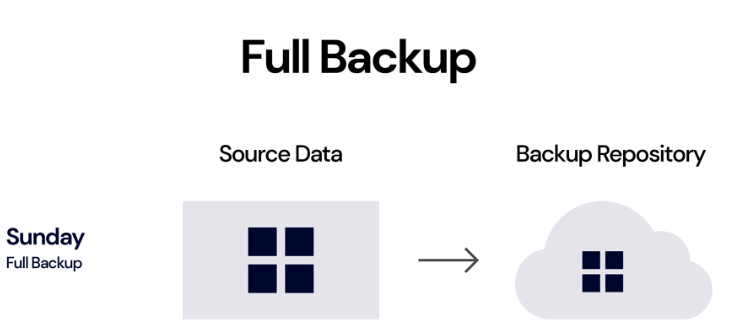
\includegraphics[width=\textwidth]{img/fullb.png}  
    \caption{Representatie van een full back-up \autocite{Rivas2022}}   
    \label{fig:fullback-up}           
\end{figure}
Een full back-up is een back-upmethode waarbij alle gegevens van een systeem op een specifiek moment volledig worden gekopieerd en opgeslagen. Dit betekent dat elk bestand zonder uitzonderingen wordt gekopieerd, zodat er een exacte kopie van de volledige dataset ontstaat \autocite{Beard2018}. Wanneer er zich een probleem voordoet, zoals het falen van een harde schijf, kan het hele bestandssysteem vanaf deze back-up volledig worden hersteld op een nieuwe schijf. Daarnaast kunnen ook individuele bestanden die verloren zijn gegaan, gemakkelijk worden teruggehaald uit de back-up. Dit soort back-up zorgt ervoor dat alle gegevens veilig zijn opgeslagen \autocite{Chervenak1998}. Full back-ups vormen vaak de basis van een back-upstrategie en worden regelmatig uitgevoerd om ervoor te zorgen dat alle gegevens volledig hersteld kunnen worden. Het concept en de implementatie van een full back-up is relatief eenvoudig omdat alle gegevens op één locatie zijn opgeslagen. Aan de andere kant is er het probleem van opslagcapaciteit. Stel bijvoorbeeld dat een bedrijf elke nacht een full back-up maakt van zijn servers naar een cloudopslagdienst, waarbij per keer 500 GB aan data wordt opgeslagen. Na een week is er al 3,5 terabyte aan gegevens in de cloud opgeslagen. Aangezien cloudproviders vaak kosten in rekening brengen op basis van gebruikte opslagcapaciteit en dataverkeer, kan dit snel leiden tot aanzienlijke maandelijkse kosten. Bedrijven met een beperkt IT-budget kunnen hierdoor in de problemen komen of worden gedwongen om strenger te selecteren welke gegevens ze precies opslaan in de back-up, omdat de opslagkosten oplopen naarmate de hoeveelheid opgeslagen data toeneemt. Daarbij kan het proces zelf ook veel tijd innemen. Dit kan voor problemen zorgen bij bedrijven waarbij de systemen aan moeten blijven. Vaak worden full back-ups gecombineerd met andere back-upmethodes. Daarnaast kost een full back-up veel tijd, wat een uitdaging kan zijn in omgevingen waar snelle gegevensbeschikbaarheid nodig is. Stel bijvoorbeeld dat een groot bedrijf tijdens kantooruren een full back-up wil maken van alle gegevens. Omdat deze back-up meerdere uren in beslag kan nemen, worden de systemen gedurende die tijd zwaar belast. Dit kan ertoe leiden dat andere processen vertraging oplopen of dat de server tijdelijk minder goed beschikbaar is voor werknemers die ook van die systemen afhankelijk zijn voor hun dagelijkse taken. Vanwege deze nadelen is het vaak beter om full back-ups aan te vullen met andere methoden \autocite{Nelson2011}.

\subsubsection{Incrementele back-up}
\begin{figure}[h] 
    \centering
    \captionsetup{justification=centering}
    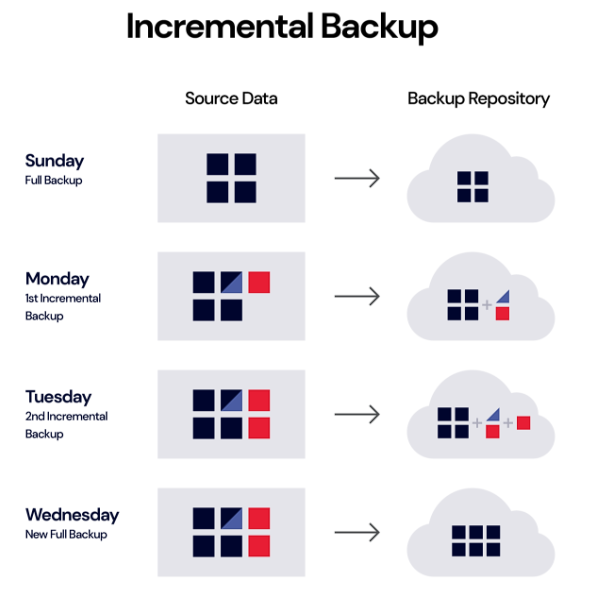
\includegraphics[width=0.5\textwidth]{img/incrementb.png}  
    \caption{Representatie van een incremental back-up \autocite{Rivas2022}}   
    \label{fig:incrback-up}           
\end{figure}

Een incrementele back-upstrategie houdt in dat na een initiële full back-up slechts de gegevens worden opgeslagen die sinds de laatste back-up zijn gewijzigd \autocite{Zhao2024}. Dit betekent dat een incrementele back-up alleen de veranderingen in de bestanden opneemt, in plaats van telkens een volledige kopie te maken van alle gegevens. Dit is vooral handig voor bedrijven die relatief vaak back-ups moeten maken, maar de opslag- en tijdskosten van een full back-up willen vermijden. Bijvoorbeeld, stel dat een bedrijf op maandag een full back-up uitvoert met al hun gegevens. Op dinsdag doet het bedrijf een incrementele back-up, waarbij enkel de wijzigingen sinds maandag worden opgeslagen. Dit gaat elke dag zo verder, elke dag wordt enkel de nieuwe of gewijzigde data opgeslagen ten opzichte van de dag ervoor. Omdat bedrijven steeds meer data beheren, biedt deze methode een efficiënte manier om opslagkosten te beperken, vooral wanneer gebruik wordt gemaakt van een cloudservice. Stel dat een bedrijf dagelijks slechts 1\% van zijn gegevens wijzigt; in plaats van elke dag een volledige kopie van bijvoorbeeld 1 TB te maken, slaat een incrementele back-up slechts de nieuwe 1\% op, wat 990 GB aan opslagruimte per dag bespaart. Dit maakt incrementele back-ups heel aantrekkelijk voor bedrijven die grote hoeveelheden data verwerken en frequente back-ups willen uitvoeren. Naast de besparing op opslagcapaciteit, zorgen incrementele back-ups voor kortere back-uptijden omdat alleen de gewijzigde bestanden worden opgeslagen. Dit betekent dat bedrijven vaker back-ups kunnen uitvoeren zonder hun systemen te vertragen. Een mediabedrijf dat met grote bestanden werkt, kan hierdoor bijvoorbeeld elk uur een incrementele back-up maken, in plaats van dagelijks een volledige back-up. Dit minimaliseert het risico op dataverlies, omdat in het geval van een storing, slechts maximaal een uur aan data verloren gaat in plaats van een hele dag. Hoewel incrementele back-ups voordelen bieden op het gebied van opslag en back-uptijden, brengen ze ook nadelen met zich mee, zoals langere hersteltijden \autocite{Chervenak1998}. Om een systeem te herstellen, heb je de laatste volledige back-up en alle volgende incrementele back-ups nodig en dit kan veel tijd kosten. Een financiële instelling die bijvoorbeeld op vrijdag een een systeemherstel moet uitvoeren, zal de volledige back-up van maandag plus alle incrementele back-ups tot en met donderdag moeten doorlopen. Dit kan relatief lang duren, wat leidt tot langere downtime, vooral in een noodsituatie waarin snelle hersteltijd van belang is. Een ander nadeel is de complexiteit van het beheer. Elke incrementele back-up hangt af van de vorige, wat betekent dat een fout in één back-up de hele herstelketen kan verstoren. Een IT-bedrijf dat dagelijks incrementele back-ups maakt, kan bijvoorbeeld problemen ondervinden als de back-up van woensdag beschadigd blijkt te zijn. Alle latere back-ups zijn afhankelijk van die ene back-up, wat het herstelproces moeilijker maakt. Dit vraagt om extra monitoring en beheer, zodat eventuele beschadigingen of herstelproblemen tijdig kunnen worden opgemerkt en opgelost.
\subsubsection{Differentiële back-ups}
\begin{figure}[h]
    \centering
    \captionsetup{justification=centering}
    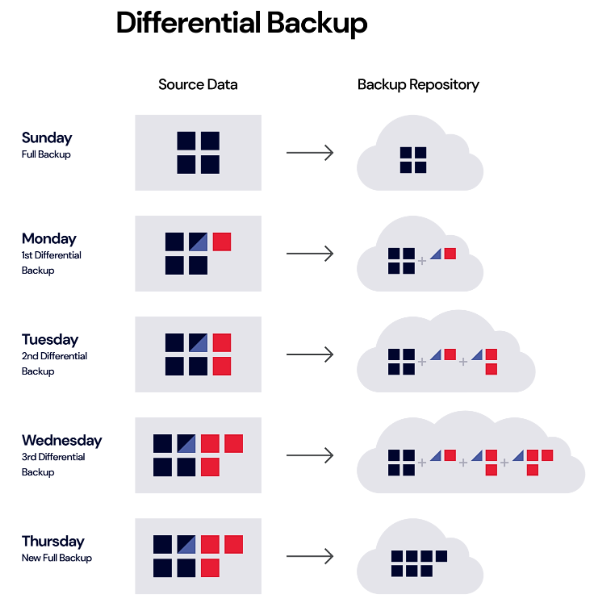
\includegraphics[width=0.5\textwidth]{img/diff.png}  
    \caption{Representatie van een differentiële back-up \autocite{Rivas2022}}   
    \label{fig:diffrback-up}           
\end{figure}
Een differentiële back-up is een soort back-up waarbij enkel de data die sinds de laatste full back-up is veranderd of toegevoegd, wordt gekopieerd. In tegenstelling tot een incrementele back-up, die enkel de veranderingen sinds de laatste back-up opslaat, wordt er bij een differentiële back-up enkel de wijzigingen opgeslagen sinds de laatste full back-up \autocite{Zhu2015}. Een differentiële back-up zal dus elke keer groter en groter worden naarmate er meer wijzigingen zijn omdat elke wijziging sinds de full back-up opgeslagen wordt. Een eerste voordeel van deze soort back-up is dat er in het geval van een recovery slechts twee back-ups nodig zijn: de laatste full back-up en de meest recente differentiële back-up. Wanneer hersteltijden belangrijk zijn zullen differentiële back-ups dus handig zijn. Bijvoorbeeld, een organisatie die dagelijks een differentiële back-up uitvoert, heeft na een week slechts de volledige back-up van de eerste dag en de laatste differentiële back-up nodig om alles te herstellen. Dit zorgt voor een relatief eenvoudig en snel herstelproces. Incrementele back-ups daarentegen slaan alleen de veranderingen op die sinds de laatste back-up zijn gemaakt van eender welke soort, of het nu een volledige of incrementele back-up is. Hierdoor zijn incrementele back-ups meestal kleiner en sneller uit te voeren dan differentiële back-ups, omdat ze alleen de allerlaatste wijzigingen bevatten. Een eerder besproken nadeel is echter dat bij herstel alle opeenvolgende back-ups nodig zijn om de data volledig terug te zetten: de laatste volledige back-up en alle incrementele back-ups tot de meest recente back-up. Dit maakt incrementele back-ups soms trager en complexer bij recovery, omdat elk back-upbestand moet worden doorlopen. Een voorbeeld om het verschil tussen incrementele back-ups en differentiële back-ups duidelijk te maken: stel dat een bedrijf aan het begin van de week een volledige back-up maakt. Bij het gebruik van een differentieel back-upschema zou elke back-up in de loop van de week groter worden, omdat elke back-up alle wijzigingen sinds die eerste dag bevat. Bij een incrementeel schema daarentegen blijft elke dagelijkse back-up klein, omdat elke nieuwe back-up alleen de nieuwste wijzigingen bevat. Als het systeem aan het einde van de week moet worden hersteld, zou met een differentieel schema enkel de full back-up en de laatste differentiële back-up nodig zijn. Bij het gebruik van incrementele-backups zijn alle back-ups van de week vereist \autocite{Beard2018}.

\subsubsection{Cloud back-ups}
Cloud back-ups zijn een populaire methode waarbij data op externe servers wordt opgeslagen, beheerd door een derde partij. In plaats van lokale fysieke opslagapparaten te gebruiken, worden de gegevens overgebracht naar een cloud-omgeving, zoals die van Amazon Web Services, Microsoft Azure of Google Cloud. Cloud back-ups bieden verschillende voordelen, zoals schaalbaarheid, eenvoud in beheer en de mogelijkheid om gegevens veilig op afstand op te slaan \autocite{Rahumed2011}. Bedrijven hoeven hierdoor geen geld te investeren in fysiek hardware. Stel dat een bedrijf snel groeit of opeens veel meer data heeft, dan kan het makkelijk zijn cloud-opslag uitbreiden zonder de IT-infrastructuur aan te passen wat veel geld en moeite zou kosten. Een van de belangrijkste voordelen van cloud back-ups is toegankelijkheid. Aangezien de gegevens zich op een externe server bevinden, kan een bedrijf op elk moment en vanaf elke locatie toegang krijgen tot zijn data, zolang er een internetverbinding is. Dit is vooral handig voor bedrijven die meerdere fysieke locaties hebben. Stel dat een bedrijf op internationaal vlak actief is: de medewerkers kunnen overal ter wereld op dezelfde back-ups vertrouwen die up-to-date zijn, dit zorgt voor een soepele samenwerking en helpt de continuïteit van het bedrijf zelfs in geval van nood. Daarnaast biedt cloud-opslag een hoge mate van beveiliging, aangezien cloud-providers meestal robuuste beveiligingsprotocollen implementeren, zoals encryptie, firewalls en multi-factor authenticatie. Voor relatief kleine bedrijven betekent dit dat zij kunnen profiteren van een hoger beveiligingsniveau zonder te investeren in geavanceerde beveiligingsinfrastructuur. Stel dat een middelgroot marketingbureau zijn klantgegevens in de cloud opslaat; de back-ups zijn dan beschermd tegen onvoorziene omstandigheden, zoals fysieke schade aan hun eigen kantoren. Echter, cloud back-ups hebben ook nadelen, waaronder de afhankelijkheid van een stabiele internetverbinding. Omdat cloud back-ups vereisen dat data over het internet wordt verzonden, kunnen problemen met de internetverbinding de back-uptijd vertragen of de overdracht volledig onderbreken. Voor een organisatie die bijvoorbeeld grote hoeveelheden videobestanden moet opslaan, kan dit tijdsverlies betekenen, vooral wanneer zij gevestigd zijn op een locatie met beperkte bandbreedte. Dit kan een probleem vormen wanneer er een strikte back-upfrequentie vereist is. Een ander nadeel is de kostprijs, vooral wanneer grote hoeveelheden gegevens vaak worden geüpdatet en opgeslagen \autocite{Obrutsky2016}. Cloud-providers vergoeden meestal de hoeveelheid opslagruimte, het dataverkeer en extra functies zoals betere encryptie of de frequentie van de back-ups. Voor een bedrijf dat veel wijzigingen aanbrengt in grote databases, zoals een online retailer met dagelijks nieuwe productinformatie, kunnen de maandelijkse kosten aanzienlijk oplopen. Dit maakt het noodzakelijk om een weloverwogen keuze te maken over de frequentie en omvang van back-ups om de kosten beheersbaar te houden. Tot slot biedt de cloud niet altijd dezelfde mate van controle als on-premise oplossingen. Hoewel cloudproviders doorgaans goede service garanderen, blijft het bedrijf afhankelijk van de beschikbaarheid en het onderhoudsbeleid van de provider. Dit betekent dat, in het geval van een storing bij de cloudprovider, bedrijven geen directe toegang hebben tot hun eigen back-ups. Een juridische firma die vertrouwelijke documenten in de cloud opslaat, kan bijvoorbeeld beperkte toegang hebben tot deze gegevens als de cloudprovider technische problemen ondervindt. Dit benadrukt het belang van goed service level agreements (SLA's) en mogelijk zelfs een hybride strategie die cloudopslag combineert met een bepaalde vorm van lokale back-ups om het risico te spreiden.

\subsubsection{On-premise back-ups}
On-premise back-ups zijn lokale back-ups die op fysieke servers binnen het bedrijf zijn opgeslagen. Het bedrijf is dus zelf verantwoordelijk voor het beheer, de beveiliging en het onderhoud van de back-upomgeving \autocite{Trovato2019}. Dit biedt bedrijven vrijheid en flexibiliteit, maar vereist wel een hoger niveau van technische kennis en onderhoud. On-premise back-ups bieden volledige controle over de gegevens, wat vooral belangrijk is in sectoren waar veiligheid en privacy cruciaal zijn, zoals de gezondheidszorg en financiële sector. Een groot voordeel is dat er geen nood is aan het internet, waardoor de snelheid van het back-upproces afhangt van de hardware dat het bedrijf bezit. Dit is ideaal voor bedrijven die snel grote hoeveelheden data moeten opslaan. Toch hebben on-premise back-ups ook nadelen. Ze vereisen een hoge initiële investering in hardware en onderhoud, zoals servers en netwerkinfrastructuur. Daarnaast zijn ze kwetsbaar voor fysieke risico’s zoals brand, diefstal of natuurrampen, wat vraagt om extra beveiligingsmaatregelen, zoals off-site back-ups. Daarbij is er ook een IT-expert nodig voor de implementatie van deze back-upsystemen, dit is soms moeilijk voor kleinere organisaties die geen speciale IT-expert hebben die dit kan doen.

\subsection{Ransomware}
Ransomware is een groeiende dreiging dat ervoor kan zorgen dat bedrijven hun gegevens voor een bepaalde tijd kwijt zijn of in het slechtste geval voor altijd kwijt zijn. Daarom moeten bedrijven zich sterk inzetten op het implementeren van een sterke back-upstrategie. Back-ups zijn het laatste redmiddel tegen ransomware-aanvallen, omdat ze een veilige kopie van data kunnen herstellen zonder te doen wat de aanvallers willen. Ransomware is een type malware dat data vergrendelt of de toegang tot gegevens blokkeert door middel van privé-sleutel encryptie, totdat er losgeld wordt betaald, meestal in Bitcoin \autocite{Richardson2017}. Malware is een softwareprogramma dat opzettelijk voldoet aan de schadelijke bedoelingen van kwaadwillende aanvallers \autocite{Yanfang2017}. Deze aanvallen kunnen niet alleen bestanden versleutelen, maar soms ook volledige systemen blokkeren, waardoor de toegang tot cruciale data verloren gaat. De gevolgen zijn vaak ernstig, omdat slachtoffers pas weer controle krijgen als ze aan de eisen van de aanvallers voldoen. Zelfs wanneer het losgeld betaald wordt, is er geen garantie dat de toegang wordt hersteld of dat de gegevens niet zijn beschadigd. Het betalen van de criminelen biedt echter geen garantie voor de toegang van de data en dit kan eindigen in een eindeloze cirkel waarbij de aanvaller elke keer opnieuw geld vraagt.

\subsubsection{Evolutie}
De evolutie van ransomware laat een gestage groei zien sinds het einde van de jaren '80. In 1989 verscheen het eerste ransomwarevirus, de AIDS Trojan, die eenvoudige versleuteling gebruikte. In 2005 kwam de moderne ransomware met Trojan.Gpcoder, die nog zwakke encryptie toepaste. Vanaf 2006 nam de populariteit van ransomware toe, met varianten zoals Trojan.Cryzip en Trojan.Archiveus. Rond 2011 begon ransomware wereldwijd uit te breiden dankzij anonieme betalingsdiensten. In 2013 werd CryptoLocker gelanceerd, een beruchte ransomware die complexe encryptie gebruikte en grote sommen losgeld eiste. Dit leidde tot een explosieve groei in ransomware-aanvallen en verfijnde technieken. Tegen 2016 bereikte ransomware een piek, waarbij het zich richtte op meerdere platformen, waaronder Linux en MacOS, en geavanceerdere strategieën gebruikte om detectie te vermijden en meer schade aan te richten. Een belangrijk aspect van deze evolutie was de introductie van Bitcoin als betaalmethode voor losgeld. De anonimiteit van Bitcoin-transacties maakte het moeilijker voor autoriteiten om aanvallers te traceren, wat bijdroeg aan de populariteit van ransomware. Bitcoin werd snel de standaard valuta voor losgeldbetalingen, wat leidde tot een verdere toename van ransomware-aanvallen. De inzet van cryptocurrencies zoals Bitcoin blijft een cruciaal onderdeel in de succesvolle verspreiding van moderne ransomware \autocite{Richardson2017}.

\subsubsection{Impact van ransomware op organisaties}
Ransomware-aanvallen hebben een aanzienlijke impact op organisaties. Ten eerste is er de financiële schade, die kan oplopen door gegevensverlies, dure herstelprocessen en de mogelijke betaling van losgeld. Naast directe kosten kunnen bedrijven ook te maken krijgen met verloren klantenvertrouwen en juridische gevolgen, wat de financiële impact verder vergroot. Ten tweede zorgen ransomware-aanvallen voor operationele verstoringen: systemen worden vaak volledig vergrendeld, wat leidt tot stilstand van cruciale bedrijfsprocessen en verlies van productieve tijd. Deze verstoringen kunnen ernstige gevolgen hebben, vooral in sectoren waar tijdige toegang tot gegevens essentieel is. Tot slot kunnen dergelijke aanvallen aanzienlijke gevolgen hebben voor de reputatie van een organisatie. Een aanval kan publieke bezorgdheid en wantrouwen opwekken, vooral als gevoelige klantinformatie wordt gelekt \autocite{Connolly2020}.

\subsection{Ransomware-resistente back-upoplossingen}
\subsubsection{Immutable storage}
Immutable storage is een techniek waarbij opgeslagen gegevens na het opslaan niet kunnen worden gewijzigd of verwijderd gedurende een vooraf vastgelegde periode. Dit zorgt voor een sterke bescherming tegen ransomware-aanvallen omdat de opgeslagen data niet meer kan worden aangepast \autocite{Wahl2023}. Het concept van immutable storage komt vooral van pas bij organisaties die te maken hebben met zeer gevoelige gegevens en die moeten kunnen garanderen dat hun data altijd veilig en betrouwbaar blijft. Één van de grootste uitdagingen is opslagcapaciteit. In een immutable opslagomgeving blijven gegevens permanent behouden, zelfs als ze verouderd of onnodig zijn. Dit zorg ervoor dat er meer opslagruimte nodig is en dit verhoogt de kosten. Een tweede nadeel heeft te maken met data throughput. Data throughput is de snelheid waarmee data kan worden overgedragen of verwerkt binnen een bepaald tijdsperiode \autocite{Miao2016}. Immutable opslag kan trager zijn bij het schrijven van gegevens omdat de immutability extra processen vereist om ervoor te zorgen dat data niet kan worden aangepast. Dit kan de snelheid van gegevensoverdracht vertragen, vooral bij systemen die software-gebaseerde immutability gebruiken, waar een extra laag van computationele controle nodig is. Ten derde zorgt het implementeren  van immutable storage vaak voor een verhoogde management overhead. Hoe meer opgeslagen data er is, hoe complexer het is om dit te beheren. Administrators moeten hierdoor meer tijd en middelen besteden aan het onderhouden van een efficiënt en veilig opslagbeheer. Ten vierde kan beveiliging ook een aandachtspunt zijn in het geval dat de er met fysieke opslagapparaten gewerkt wordt. Bij software-gebaseerde immutability kan er sprake zijn van gevaar indien het hele besturingssysteem is aangevallen. Ten slotte kunnen de kosten snel oplopen. De initiële investering in immutable opslag kan hoog zijn, vooral als er gekozen wordt voor dure opslagmedia of gespecialiseerde hardware. Naarmate de hoeveelheid gegevens toeneemt, nemen ook de kosten voor opslag en onderhoud toe \autocite{Hasan2005}.

\subsubsection{Air-gapped storage}
Air-gapped back-ups bieden sterke bescherming tegen ransomware door back-ups fysiek of virtueel te isoleren van het netwerk. Dit betekent dat, zelfs als het netwerk wordt aangevallen, de back-ups veilig blijven omdat ze niet verbonden zijn met de geïnfecteerde systemen. Deze back-ups worden vaak opgeslagen op externe media zoals harde schijven \autocite{Bryant2015}. Air-gapping zorgt ervoor dat het onmogelijk is voor ransomware om de back-ups te infecteren, waardoor een bedrijf snel kan herstellen van een aanval en de bedrijfscontinuïteit kan behouden. Het maakt bedrijven minder afhankelijk van cloud-opslag en netwerkverbindingen, wat de risico’s vermindert. Hoewel air-gapped back-ups een goede bescherming bieden tegen ransomware, kunnen ze minder snel toegankelijk zijn wanneer gegevensherstel nodig is. Deze back-ups moeten namelijk fysiek worden opgehaald en aangesloten, wat veel tijd kan kosten. Desondanks bieden air-gapped back-ups een extra laag van beveiliging die van groot belang is voor organisaties die gevoelig zijn voor ransomware-aanvallen \autocite{Park2023}.

\subsubsection{Offline back-ups}
Offline back-ups worden opgeslagen op externe media zoals harde schijven die na het back-uppen van het netwerk worden losgekoppeld\autocite{Edwards2022}. Dit maakt ze immuun voor online bedreigingen zoals ransomware, in tegenstelling tot on-premise back-ups die meestal verbonden blijven met het netwerk. Het grootste voordeel van offline back-ups is de extra beveiliging tegen cyberaanvallen, aangezien ze fysiek losgekoppeld zijn en daardoor buiten bereik van hackers blijven. Dit biedt bedrijven met gevoelige gegevens, zoals advocatenkantoren, een betrouwbare manier om data te beschermen tegen digitale bedreigingen. Een ander voordeel is de fysieke controle over de opslaglocatie, waardoor bedrijven precies kunnen bepalen wie toegang heeft tot de gegevens. Toch hebben offline back-ups ook nadelen: ze moeten handmatig worden bijgewerkt, wat tijdrovend is, en zijn kwetsbaar voor fysieke schade zoals brand of diefstal. Daarnaast kan het herstelproces langer duren, omdat de gegevens fysiek aangesloten en overgezet moeten worden, wat minder efficiënt is voor bedrijven die snel dataherstel nodig hebben \autocite{James2019}.

\subsection{Technologische basis voor de Proof-of-Concept}
Voor de Proof-of-Concept wordt gebruik gemaakt van verschillende technologische tools en platforms. Deze worden ingezet om de geplande back-upstrategie en de beveiligingsmaatregelen te testen en te optimaliseren. Hierbij wordt specifiek gewerkt met tools zoals Azure, VirtualBox en Vagrant. Deze technologieën worden gekozen vanwege hun flexibiliteit, schaalbaarheid en ondersteuning bij het simuleren van realistische scenario's.
\subsubsection{Azure}
Azure wordt gezien als het openbare cloudplatform van Microsoft en maakt gebruik van virtualisatietechnologie \autocite{Ekuan2023}. Door middel van virtualisatietechnologieën, ook wel hypervisors genoemd (Een hypervisor is software waarmee meerdere virtuele machines (VM's), elk met hun eigen besturingssysteem (OS), op één fysieke server kunnen draaien \autocite{Susnjara2024}.), is het mogelijk voor Azure om hardware na te bootsen in software. Dit gebeurt in datacenters die zijn opgebouwd uit serverrekken met onder andere netwerkswitches en voldoende stroomvoorzieningen. Binnen een Azure-datacenter bevinden zich serverrekken, die elk uit meerdere serverblades bestaan. Deze serverrekken bevatten ook netwerkhardware, zoals netwerkswitches, en een PDU (Power Distribution Unit), die stroomvoorziening biedt. Voor extra schaalbaarheid en efficiëntie worden deze serverrekken vaak gegroepeerd in clusters. Servers met speciale software, zoals infrastructuurcontrollers, zorgen ervoor dat services efficiënt worden toegewezen en storingen worden opgelost. Azure is meer dan alleen een verzameling servers. Het is een complex netwerk van toepassingen die samenwerken om gevirtualiseerde hardware en software te configureren en beheren. Dit maakt Azure een krachtig en flexibel platform voor gebruikers.

Azure Blob Storage is de objectopslagoplossing van Microsoft voor de cloud, geoptimaliseerd voor het opslaan van grote hoeveelheden ongestructureerde data \autocite{Dubey2023}. Azure Blob Storage biedt immutable storage in een WORM-status (Write Once, Read Many), waarmee data niet kan worden aangepast of verwijderd gedurende een ingestelde periode. Dit is ideaal voor sectoren met strenge nalevingsvereisten, zoals financiën en gezondheidszorg.  Er zijn twee immutability policies beschikbaar:

\begin{itemize}[leftmargin=1cm]
    \item \textbf{Tijdgebonden retentiebeleid:} Data blijft gedurende een specifieke periode onveranderlijk. Na afloop kunnen bestanden worden verwijderd, maar niet overschreven. Dit beleid kan op account-, container- of versieniveau worden toegepast en kan van ``unlocked'' naar ``gelocked'' worden gezet voor naleving van regelgeving. Eenmaal gelocked, kan de retentieperiode alleen worden verlengd.
    \item \textbf{Legal holds:} Houdt data onveranderlijk tot de hold expliciet wordt opgeheven. Dit is nuttig bij onbepaalde bewaartermijnen, zoals juridische onderzoeken, en kan worden toegepast op container- of blobversieniveau \autocite{Estabrook2024}.
\end{itemize}
Azure ondersteunt immutability op twee vb niveaus: container-level, waarbij alle blobs in een container hetzelfde beleid volgen, en version-level, dat flexibiliteit biedt voor individuele blobs met verschillende retentievereisten. Een blob (Binary Large Object) is een type dataopslag dat gebruikt wordt om grote hoeveelheden ongestructureerde gegevens op te slaan, zoals tekst, afbeeldingen, video's, audio of binaire bestanden \autocite{Kemp2007}. Samen zorgen deze opties voor veilige en conforme opslag.



\subsubsection{Vagrant}
Vagrant is een open-source tool ontwikkeld door HashiCorp die het proces van het beheren en configureren van virtuele machines automatiseert \autocite{Hashicorp}. HashiCorp is een bedrijf dat tools maakt voor infrastructuurbeheer. 

Het zorgt ervoor dat gebruikers virtuele machines snel kunnen creëren en configureren door gebruik te maken van gestandaardiseerde configuratiebestanden, genaamd Vagrantfiles. In de Vagrantfiles kun je allerlei configuraties kiezen zoals netwerkconfiguraties, besturingssystemen en softwarepakketten. Het biedt ondersteuning voor verschillende virtualisatieplatforms, zoals VirtualBox, VMware en Hyper-V, en kan worden geïntegreerd met provisioning-tools zoals Ansible. Vagrant wordt vaak gebruikt voor het opzetten van test- en ontwikkelomgevingen.

\subsubsection{Virtualbox}
VirtualBox is een open-source virtualisatiesoftware die ervoor zorgt dat gebruikers meerdere besturingssystemen tegelijkertijd op één fysieke machine kunnen draaien \autocite{Oracle}. Virtualbox biedt veel functionaliteiten aan, waaronder ondersteuning voor diverse gastbesturingssystemen zoals Windows en Linux, daarnaast zijn de netwerkconfiguraties ook geavanceerd. VirtualBox maakt gebruik van virtuele netwerken, zoals NAT (Network Address Translation) en interne netwerken, waarmee gebruikers flexibele en gescheiden infrastructuren kunnen opzetten. Dankzij de grafische interface en command-line tools is het een toegankelijk platform voor zowel beginners als gevorderde IT-professionals. Daarbij is VirtualBox geschikt voor allerlei doelen zoals softwareontwikkeling, systeembeheer en educatieve simulaties voor scholen.

\subsubsection{BorgBackup}

\subsubsection{MySQL}
%%=============================================================================
%% Methodologie
%%=============================================================================

\chapter{\IfLanguageName{dutch}{Methodologie}{Methodology}}%
\label{ch:methodologie}

%% TODO: In dit hoofstuk geef je een korte toelichting over hoe je te werk bent
%% gegaan. Verdeel je onderzoek in grote fasen, en licht in elke fase toe wat
%% de doelstelling was, welke deliverables daar uit gekomen zijn, en welke
%% onderzoeksmethoden je daarbij toegepast hebt. Verantwoord waarom je
%% op deze manier te werk gegaan bent.
%% 
%% Voorbeelden van zulke fasen zijn: literatuurstudie, opstellen van een
%% requirements-analyse, opstellen long-list (bij vergelijkende studie),
%% selectie van geschikte tools (bij vergelijkende studie, "short-list"),
%% opzetten testopstelling/PoC, uitvoeren testen en verzamelen
%% van resultaten, analyse van resultaten, ...
%%
%% !!!!! LET OP !!!!!
%%
%% Het is uitdrukkelijk NIET de bedoeling dat je het grootste deel van de corpus
%% van je bachelorproef in dit hoofstuk verwerkt! Dit hoofdstuk is eerder een
%% kort overzicht van je plan van aanpak.
%%
%% Maak voor elke fase (behalve het literatuuronderzoek) een NIEUW HOOFDSTUK aan
%% en geef het een gepaste titel.

\lipsum[21-25]



% Voeg hier je eigen hoofdstukken toe die de ``corpus'' van je bachelorproef
% vormen. De structuur en titels hangen af van je eigen onderzoek. Je kan bv.
% elke fase in je onderzoek in een apart hoofdstuk bespreken.

\chapter{\IfLanguageName{dutch}{literatuurstudie}{Introduction}}%
\label{ch:Literatuurstudie}

\subsection{Back-ups in het kader van bedrijfscontinuïteit en disaster recovery}
Bedrijfscontinuïteit verwijst naar de aanpak en procedures dat een bedrijf gebruikt om de voortgang van zijn werkzaamheden te bewaren, zelfs in het geval van incidenten. Deze incidenten kunnen variëren van relatief kleine problemen, zoals een gebroken netwerkverbinding, tot grote natuurrampen zoals een aardbevingen. Omdat er zoveel soorten incidenten kunnen gebeuren is het moeilijk om een oplossing te vinden die ervoor zorgt dat bedrijven in alle gevallen beschermt zijn. In plaats daarvan gebruiken bedrijven een mix van strategieën en technologieën om de continuïteit van hun processen te beschermen. De 2 belangrijkste concepten voor de bedrijfscontinuïteit zijn hoge beschikbaarheid en disaster recovery. Hoge beschikbaarheid duidt op het feit dat een bedrijf zodanig is ingericht dat het kan blijven draaien, zelfs als bepaalde systemen of componenten uitvallen. Een voorbeeld hiervan zijn twee routers die zijn geconfigureerd in een actieve-passieve opstelling. In deze configuratie is één router de primaire router die al het inkomende en uitgaande verkeer verwerkt, terwijl de andere router als reserve werkt. In het geval dat de primaire router faalt door een hardwarestoringen of netwerkprobleem, dan neemt de tweede router automatisch de rol van de primaire router over, zonder dat dit merkbare impact heeft op de netwerkverbindingen van de organisatie. Hierdoor blijft de beschikbaarheid van het netwerk gegarandeerd en blijft de downtime laag \autocite{Zhu2015}. Disaster recovery (DR) is een onderdeel van bedrijfscontinuïteit dat zich specifiek richt op het herstellen van bedrijfsactiviteiten na een incident zoals een cyberaanval of ernstige verstoring. Terwijl bedrijfscontinuïteit zich richt op bredere preventieve maatregelen om de continuïteit te waarborgen, focust disaster recovery zich juist op de praktische stappen en hulpmiddelen die nodig zijn om de organisatie na een verstoring weer snel operationeel te maken. Het doel van disaster recovery is om schade zoveel mogelijk te beperken en de normale gang van zaken zo snel mogelijk te herstellen. Back-ups spelen een belangrijke rol voor de continuïteit van een bedrijf en zijn vaak de eerste stap bij het opstellen van een disaster recovery plan (DRP). Bij een optimale situatie is er na een incident geen data verloren en is alle data relatief snel terug beschikbaar. Indien een bedrijf geen back-ups heeft van de belangrijke data zal de data in het geval van een incident verloren raken. Zonder back-ups zal het ook een grotere uitdaging zijn voor het bedrijf om de normale bedrijfsactiviteiten terug uit te voeren. Een belangrijke doelstelling van een bedrijf is winst maken. In het geval van een incident waarbij de bedrijfsactiviteiten niet normaal kunnen verlopen zal deze doelstelling verhindert worden en zal er dus financieel verlies optreden. Bij specifieke bedreigingen, zoals ransomware-aanvallen spelen ransomware-resistente back-ups een cruciale rol. Door back-ups te beveiligen tegen ransomware-aanvallen kunnen bedrijven hun data herstellen zonder losgeld te betalen. Dit benadrukt het belang van back-ups die niet alleen snel toegankelijk zijn, maar ook bestand zijn tegen digitale bedreigingen \autocite{Ghazi2013}.

\subsection{Back-upmethoden en -technieken}
Back-ups zijn een belangrijk onderdeel van datamanagement en databeveiliging binnen organisaties. Back-ups zorgen voor de continuïteit van bedrijfssystemen in het geval van een incident zoals een cyberaanval. Back-ups zijn snapshots van gegevens die op een bepaald tijdstip zijn gemaakt, opgeslagen in een wereldwijd gebruikelijk formaat en gedurende een bepaalde periode van bruikbaarheid worden bijgehouden, waarbij elke volgende kopie van de gegevens onafhankelijk van de eerste wordt bewaard\autocite{Nelson2011}. Door een aparte kopie van de gegevens te bewaren, kunnen bedrijven en individuen na een incident hun systemen of bestanden herstellen naar een eerdere, veilige staat. Hierbij kunnen back-ups zowel volledige datasets als selectieve bestandstypen omvatten, afhankelijk van de strategie en de specifieke behoeften van de organisatie. Back-ups zijn een preventieve maatregel en het doel ervan is om dataverlies tegen te gaan. Dataverlies kan optreden door menselijke fouten, cyberaanvallen, en natuur- of bedrijfsrampen. Daarbij speelt beveiliging een belangrijke rol in een tijd waarin ransomware-aanvallen en datalekken frequenter voorkomen. Door back-ups versleuteld op te slaan en te beveiligen tegen ongeautoriseerde toegang, kunnen bedrijven zich beschermen tegen het verliezen van data. 
\subsubsection{Full back-ups}
\begin{figure}[h] 
    \centering
    \captionsetup{justification=centering}
    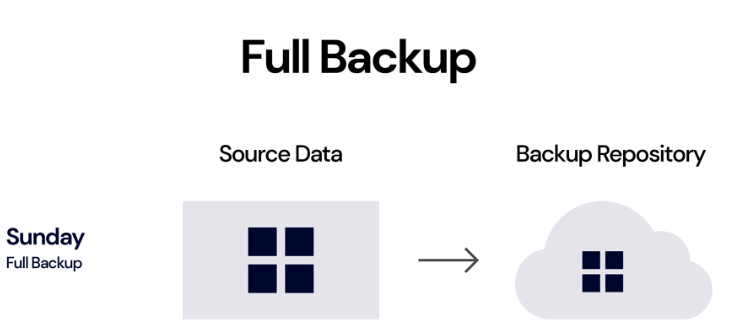
\includegraphics[width=\textwidth]{img/fullb.png}  
    \caption{Representatie van een full back-up \autocite{Rivas2022}}   
    \label{fig:fullback-up}           
\end{figure}
Een full back-up is een back-upmethode waarbij alle gegevens van een systeem op een specifiek moment volledig worden gekopieerd en opgeslagen. Dit betekent dat elk bestand zonder uitzonderingen wordt gekopieerd, zodat er een exacte kopie van de volledige dataset ontstaat \autocite{Beard2018}. Wanneer er zich een probleem voordoet, zoals het falen van een harde schijf, kan het hele bestandssysteem vanaf deze back-up volledig worden hersteld op een nieuwe schijf. Daarnaast kunnen ook individuele bestanden die verloren zijn gegaan, gemakkelijk worden teruggehaald uit de back-up. Dit soort back-up zorgt ervoor dat alle gegevens veilig zijn opgeslagen \autocite{Chervenak1998}. Full back-ups vormen vaak de basis van een back-upstrategie en worden regelmatig uitgevoerd om ervoor te zorgen dat alle gegevens volledig hersteld kunnen worden. Het concept en de implementatie van een full back-up is relatief eenvoudig omdat alle gegevens op één locatie zijn opgeslagen. Aan de andere kant is er het probleem van opslagcapaciteit. Stel bijvoorbeeld dat een bedrijf elke nacht een full back-up maakt van zijn servers naar een cloudopslagdienst, waarbij per keer 500 GB aan data wordt opgeslagen. Na een week is er al 3,5 terabyte aan gegevens in de cloud opgeslagen. Aangezien cloudproviders vaak kosten in rekening brengen op basis van gebruikte opslagcapaciteit en dataverkeer, kan dit snel leiden tot aanzienlijke maandelijkse kosten. Bedrijven met een beperkt IT-budget kunnen hierdoor in de problemen komen of worden gedwongen om strenger te selecteren welke gegevens ze precies opslaan in de back-up, omdat de opslagkosten oplopen naarmate de hoeveelheid opgeslagen data toeneemt. Daarbij kan het proces zelf ook veel tijd innemen. Dit kan voor problemen zorgen bij bedrijven waarbij de systemen aan moeten blijven. Vaak worden full back-ups gecombineerd met andere back-upmethodes. Daarnaast kost een full back-up veel tijd, wat een uitdaging kan zijn in omgevingen waar snelle gegevensbeschikbaarheid nodig is. Stel bijvoorbeeld dat een groot bedrijf tijdens kantooruren een full back-up wil maken van alle gegevens. Omdat deze back-up meerdere uren in beslag kan nemen, worden de systemen gedurende die tijd zwaar belast. Dit kan ertoe leiden dat andere processen vertraging oplopen of dat de server tijdelijk minder goed beschikbaar is voor werknemers die ook van die systemen afhankelijk zijn voor hun dagelijkse taken. Vanwege deze nadelen is het vaak beter om full back-ups aan te vullen met andere methoden \autocite{Nelson2011}.

\subsubsection{Incrementele back-up}
\begin{figure}[h] 
    \centering
    \captionsetup{justification=centering}
    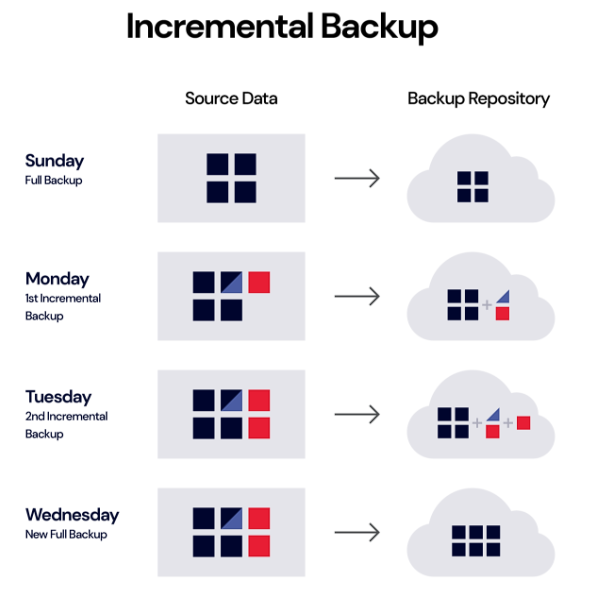
\includegraphics[width=0.5\textwidth]{img/incrementb.png}  
    \caption{Representatie van een incremental back-up \autocite{Rivas2022}}   
    \label{fig:incrback-up}           
\end{figure}

Een incrementele back-upstrategie houdt in dat na een initiële full back-up slechts de gegevens worden opgeslagen die sinds de laatste back-up zijn gewijzigd \autocite{Zhao2024}. Dit betekent dat een incrementele back-up alleen de veranderingen in de bestanden opneemt, in plaats van telkens een volledige kopie te maken van alle gegevens. Dit is vooral handig voor bedrijven die relatief vaak back-ups moeten maken, maar de opslag- en tijdskosten van een full back-up willen vermijden. Bijvoorbeeld, stel dat een bedrijf op maandag een full back-up uitvoert met al hun gegevens. Op dinsdag doet het bedrijf een incrementele back-up, waarbij enkel de wijzigingen sinds maandag worden opgeslagen. Dit gaat elke dag zo verder, elke dag wordt enkel de nieuwe of gewijzigde data opgeslagen ten opzichte van de dag ervoor. Omdat bedrijven steeds meer data beheren, biedt deze methode een efficiënte manier om opslagkosten te beperken, vooral wanneer gebruik wordt gemaakt van een cloudservice. Stel dat een bedrijf dagelijks slechts 1\% van zijn gegevens wijzigt; in plaats van elke dag een volledige kopie van bijvoorbeeld 1 TB te maken, slaat een incrementele back-up slechts de nieuwe 1\% op, wat 990 GB aan opslagruimte per dag bespaart. Dit maakt incrementele back-ups heel aantrekkelijk voor bedrijven die grote hoeveelheden data verwerken en frequente back-ups willen uitvoeren. Naast de besparing op opslagcapaciteit, zorgen incrementele back-ups voor kortere back-uptijden omdat alleen de gewijzigde bestanden worden opgeslagen. Dit betekent dat bedrijven vaker back-ups kunnen uitvoeren zonder hun systemen te vertragen. Een mediabedrijf dat met grote bestanden werkt, kan hierdoor bijvoorbeeld elk uur een incrementele back-up maken, in plaats van dagelijks een volledige back-up. Dit minimaliseert het risico op dataverlies, omdat in het geval van een storing, slechts maximaal een uur aan data verloren gaat in plaats van een hele dag. Hoewel incrementele back-ups voordelen bieden op het gebied van opslag en back-uptijden, brengen ze ook nadelen met zich mee, zoals langere hersteltijden\autocite{Chervenak1998}. Om een systeem te herstellen, heb je de laatste volledige back-up en alle volgende incrementele back-ups nodig en dit kan veel tijd kosten. Een financiële instelling die bijvoorbeeld op vrijdag een een systeemherstel moet uitvoeren, zal de volledige back-up van maandag plus alle incrementele back-ups tot en met donderdag moeten doorlopen. Dit kan relatief lang duren, wat leidt tot langere downtime, vooral in een noodsituatie waarin snelle hersteltijd van belang is. Een ander nadeel is de complexiteit van het beheer. Elke incrementele back-up hangt af van de vorige, wat betekent dat een fout in één back-up de hele herstelketen kan verstoren. Een IT-bedrijf dat dagelijks incrementele back-ups maakt, kan bijvoorbeeld problemen ondervinden als de back-up van woensdag beschadigd blijkt te zijn. Alle latere back-ups zijn afhankelijk van die ene back-up, wat het herstelproces moeilijker maakt. Dit vraagt om extra monitoring en beheer, zodat eventuele beschadigingen of herstelproblemen tijdig kunnen worden opgemerkt en opgelost.
\subsubsection{Differentiële back-ups}
 \begin{figure}[h]
    \centering
    \captionsetup{justification=centering}
    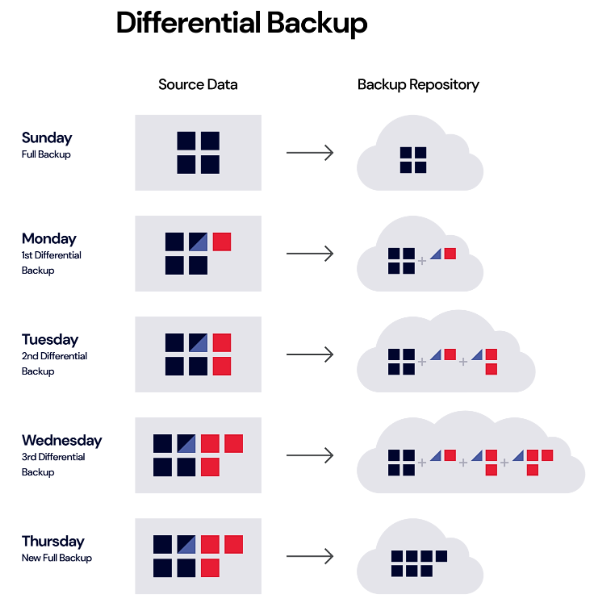
\includegraphics[width=0.5\textwidth]{img/diff.png}  
    \caption{Representatie van een differentiële back-up \autocite{Rivas2022}}   
    \label{fig:diffrback-up}           
\end{figure}
Een differentiële back-up is een soort back-up waarbij alleen de data die sinds de laatste volledige back-up is veranderd of toegevoegd, wordt gekopieerd. In tegenstelling tot een incrementele back-up, die enkel de veranderingen sinds de laatste back-up opslaat, wordt er bij een differentiële back-up enkel de wijzigingen opgeslagen sinds de laatste full back-up \autocite{Beard2018}. Dit betekent dat elke nieuwe differentiële back-up groter wordt naarmate er meer wijzigingen plaatsvinden, omdat hij telkens opnieuw alle wijzigingen sinds die laatste full back-up bevat. Een voordeel van deze aanpak is dat voor herstel slechts twee back-ups nodig zijn: de laatste volledige back-up en de meest recente differentiële back-up. Dit maakt differentiële back-ups aantrekkelijk wanneer herstelsnelheid een prioriteit is. Bijvoorbeeld, een organisatie die dagelijks een differentiële back-up uitvoert, heeft na een week slechts de volledige back-up van de eerste dag en de laatste differentiële back-up nodig om alles te herstellen. Dit zorgt voor een relatief eenvoudig en snel herstelproces. Incrementele back-ups daarentegen slaan alleen de veranderingen op die sinds de laatste back-up van welke aard dan ook zijn gemaakt, of het nu een volledige of incrementele back-up is. Hierdoor zijn incrementele back-ups meestal kleiner en sneller uit te voeren dan differentiële back-ups, omdat ze alleen de allerlaatste wijzigingen bevatten. Een eerder besproken nadeel is echter dat bij herstel alle opeenvolgende back-ups nodig zijn om de data volledig terug te zetten: de laatste volledige back-up en alle incrementele back-ups tot de meest recente back-up. Dit maakt incrementele back-ups soms trager en complexer bij herstel, omdat elk back-upbestand moet worden doorlopen. Een voorbeeld om het verschil tussen incrementele back-ups en differentiële back-ups duidelijk te maken: stel dat een bedrijf aan het begin van de week een volledige back-up maakt. Bij het gebruik van een differentieel back-upschema zou elke back-up in de loop van de week groter worden, omdat elke back-up alle wijzigingen sinds die eerste dag bevat. Bij een incrementeel schema daarentegen blijft elke dagelijkse back-up klein, omdat elke nieuwe back-up alleen de nieuwste wijzigingen bevat. Als het systeem aan het einde van de week moet worden hersteld, zou met een differentieel schema slechts de volledige back-up en de laatste differentiële back-up nodig zijn. Bij het incrementele schema zijn echter alle back-ups van de week vereist.

\subsubsection{Cloud back-ups}
Cloud back-ups zijn een populaire methode waarbij data op externe servers wordt opgeslagen, beheerd door een derde partij. In plaats van lokale fysieke opslagapparaten te gebruiken, worden de gegevens overgebracht naar een cloudomgeving, zoals die van Amazon Web Services, Microsoft Azure of Google Cloud. Cloud back-ups bieden verschillende voordelen, zoals schaalbaarheid, eenvoud in beheer en de mogelijkheid om gegevens veilig op afstand op te slaan. Voor bedrijven betekent dit dat zij geen dure fysieke hardware hoeven aan te schaffen, en de infrastructuur flexibel kunnen aanpassen aan hun behoeften. Een bedrijf dat bijvoorbeeld snel groeit, kan zijn cloudopslag uitbreiden zonder ingrijpende veranderingen aan de interne IT-omgeving. Een van de belangrijkste voordelen van cloud back-ups is toegankelijkheid. Aangezien de gegevens zich op een externe server bevinden, kan een bedrijf op elk moment en vanaf elke locatie toegang krijgen tot zijn data, zolang er een internetverbinding is. Dit kan cruciaal zijn voor organisaties met vestigingen op meerdere locaties. Stel dat een bedrijf werkt met een gedistribueerd team: de medewerkers kunnen overal ter wereld op dezelfde up-to-date back-ups vertrouwen, wat de samenwerking vergemakkelijkt en de continuïteit waarborgt, zelfs in noodsituaties. Daarnaast biedt cloudopslag een hoge mate van beveiliging, aangezien cloudproviders meestal robuuste beveiligingsprotocollen implementeren, zoals encryptie, firewalls en multi-factor authenticatie. Voor veel kleinere bedrijven betekent dit dat zij kunnen profiteren van een hoger beveiligingsniveau zonder te investeren in geavanceerde beveiligingsinfrastructuur. Stel dat een middelgroot marketingbureau zijn klantgegevens in de cloud opslaat; de back-ups zijn dan beschermd tegen onvoorziene omstandigheden, zoals fysieke schade aan hun eigen kantoren. Echter, cloud back-ups hebben ook nadelen, waaronder de afhankelijkheid van een stabiele internetverbinding. Omdat cloud back-ups vereisen dat data over het internet wordt verzonden, kunnen problemen met de internetverbinding de back-uptijd vertragen of de overdracht volledig onderbreken. Voor een organisatie die bijvoorbeeld grote hoeveelheden videobestanden moet opslaan, kan dit tijdsverlies betekenen, vooral wanneer zij gevestigd zijn op een locatie met beperkte bandbreedte. Dit kan een probleem vormen wanneer er een strikte back-upfrequentie vereist is. Een ander nadeel is de kostprijs, vooral wanneer grote hoeveelheden gegevens vaak worden geüpdatet en opgeslagen. Cloudopslagproviders rekenen doorgaans kosten voor opslagcapaciteit, maar ook voor dataverkeer en extra functies zoals geavanceerde encryptie of frequentere back-ups. Voor een bedrijf dat veel wijzigingen aanbrengt in grote databases, zoals een online retailer met dagelijks nieuwe productinformatie, kunnen de maandelijkse kosten aanzienlijk oplopen. Dit maakt het noodzakelijk om een weloverwogen keuze te maken over de frequentie en omvang van back-ups om de kosten beheersbaar te houden. Tot slot biedt de cloud niet altijd dezelfde mate van controle als on-premise oplossingen. Hoewel cloudproviders doorgaans goede service garanderen, blijft het bedrijf afhankelijk van de beschikbaarheid en het onderhoudsbeleid van de provider. Dit betekent dat, in het geval van een storing bij de cloudprovider, bedrijven geen directe toegang hebben tot hun eigen back-ups. Een juridische firma die vertrouwelijke documenten in de cloud opslaat, kan bijvoorbeeld beperkte toegang hebben tot deze gegevens als de cloudprovider technische problemen ondervindt. Dit benadrukt het belang van goed service level agreements (SLA's) en mogelijk zelfs een hybride strategie die cloudopslag combineert met een bepaalde vorm van lokale back-ups om het risico te spreiden.


\subsubsection{On-premise back-ups}
On-premise back-ups zijn back-ups die lokaal worden opgeslagen op de fysieke servers en opslagapparaten binnen de infrastructuur van een bedrijf. Deze methode houdt in dat het bedrijf zelf verantwoordelijk is voor het beheren, beveiligen en onderhouden van de back-upomgeving. Voor organisaties die volledige controle willen over hun gegevens, bieden on-premise back-ups een direct en tastbaar voordeel: de data blijft in eigen beheer, wat vooral waardevol is in sectoren waar data security en privacy van groot belang zijn, zoals de gezondheidszorg of financiële dienstverlening. Een van de grootste voordelen van on-premise back-ups is dat er geen afhankelijkheid is van een internetverbinding. Aangezien de back-up lokaal gebeurt, is de snelheid van het netwerk binnen het bedrijf bepalend voor de snelheid van het back-upproces. Voor een organisatie met een snelle interne netwerkinfrastructuur, zoals een mediabedrijf dat dagelijks grote videobestanden back-upt, kan dit het verschil maken tussen uren en minuten. Dit maakt on-premise back-ups een ideale keuze voor bedrijven die snel grote hoeveelheden data moeten opslaan zonder gehinderd te worden door internetbeperkingen. Daarnaast biedt on-premise opslag de mogelijkheid om de volledige back-up- en herstelstrategie te personaliseren en aan te passen aan de specifieke behoeften van de organisatie. Dit kan belangrijk zijn voor bedrijven die bepaalde compliance-eisen hebben of die willen experimenteren met specifieke back-uptechnieken, zoals differential of incremental back-ups. Een bedrijf in de financiële sector kan bijvoorbeeld ervoor kiezen om alle dagelijkse transacties lokaal op te slaan en de volledige back-ups wekelijks op een afgescheiden server te bewaren. Op deze manier kunnen zij hun data volledig beheren, met maatregelen die specifiek zijn afgestemd op hun eigen risico’s en beleid. Toch komen on-premise back-ups met aanzienlijke nadelen. Een belangrijke uitdaging is de hoge initiële investering in hardware en onderhoud. Bedrijven moeten investeren in servers, harde schijven, netwerkinfrastructuur en mogelijk zelfs koeling- en beveiligingssystemen. Voor een middelgroot productiebedrijf dat bijvoorbeeld zijn back-ups op eigen servers wil opslaan, kan dit een aanzienlijke uitgave betekenen. Bovendien moeten deze systemen regelmatig worden geüpdatet en vervangen, wat extra kosten en logistieke planning met zich meebrengt. Een ander nadeel van on-premise back-ups is dat ze gevoelig zijn voor fysieke risico’s zoals brand, diefstal of overstromingen. Aangezien de gegevens op locatie zijn opgeslagen, kunnen ze verloren gaan als de infrastructuur fysiek wordt beschadigd. Dit betekent dat bedrijven extra beveiligingsmaatregelen moeten nemen, zoals een secundaire back-up op een externe locatie. Stel dat een IT-bedrijf zijn servers in zijn hoofdkantoor opslaat en daar een brand uitbreekt; dan zijn zowel de primaire data als de back-up data in gevaar, tenzij er een tweede kopie offsite is opgeslagen. Dit vergroot de behoefte aan een goed doordachte noodherstelstrategie. Daarnaast vereisen on-premise back-ups specifieke IT-expertise om een goed beheerde en beveiligde omgeving te handhaven. Het interne IT-team moet in staat zijn om regelmatig back-ups uit te voeren, beveiligingsupdates bij te houden, en ervoor te zorgen dat de gegevens ten alle tijden toegankelijk en veilig zijn. Voor een kleine organisatie zonder een toegewijd IT-team kan dit een uitdaging zijn, aangezien deze taken continu onderhoud en aandacht vereisen.
\subsubsection{Offline back-ups}
Offline back-ups zijn back-ups die fysiek worden opgeslagen op opslagmedia zoals externe harde schijven, tape-drives of andere niet-aangesloten apparaten, zonder constante verbinding met het netwerk of internet. Het belangrijkste verschil met on-premise back-ups is dat offline back-ups na het maken ervan van het netwerk worden losgekoppeld, waardoor ze immuun worden voor online bedreigingen zoals ransomware of hacking. Bij on-premise back-ups blijven de gegevens meestal beschikbaar binnen de lokale netwerkomgeving van het bedrijf, terwijl offline back-ups juist fysiek worden verwijderd van elke vorm van netwerktoegang. Een van de grootste voordelen van offline back-ups is dat ze een extra laag bescherming bieden tegen cyberaanvallen. Doordat deze back-ups niet online toegankelijk zijn, kunnen kwaadwillenden er via het netwerk geen toegang toe krijgen. Dit kan een essentieel voordeel zijn voor bedrijven die met gevoelige gegevens werken, zoals een advocatenkantoor dat juridische documenten opslaat. Stel dat een ransomware-aanval het hele netwerk vergrendelt, dan blijven de offline back-ups onaangetast, omdat ze fysiek losgekoppeld zijn van het geïnfecteerde systeem. Op deze manier kunnen bedrijven hun gegevens nog steeds herstellen, zelfs in het geval van een grote cyberaanval. Offline back-ups bieden ook het voordeel van fysieke controle. Een bedrijf dat zijn offline back-ups in een kluis of beveiligde ruimte opslaat, heeft de zekerheid dat de gegevens veilig zijn tegen zowel digitale als sommige fysieke bedreigingen. Dit is bijvoorbeeld handig voor een onderzoeksorganisatie die vertrouwelijke onderzoeksgegevens heeft en ervoor wil zorgen dat alleen bevoegde personen toegang hebben. Door de back-ups fysiek op te slaan in een beveiligde ruimte kan worden bepaald wie wanneer bij de data kan. Echter, offline back-ups brengen ook enkele nadelen met zich mee. Een van de grootste uitdagingen is dat ze handmatig moeten worden bijgewerkt, wat arbeidsintensief kan zijn. Dit kan een probleem vormen voor bedrijven met zeer regelmatig veranderende gegevens. Neem een klein e-commercebedrijf dat elke dag nieuwe verkoopgegevens verzamelt en opslaat; om deze data te beschermen, zou dagelijks een offline back-up moeten worden gemaakt en fysiek worden opgeborgen. Dit proces kan tijdrovend zijn en vereist dat er een routine is om deze back-ups nauwgezet te beheren. Een ander nadeel van offline back-ups is dat ze kwetsbaar blijven voor fysieke schade, verlies of diefstal. Aangezien ze worden opgeslagen op fysieke media, zijn ze gevoelig voor gebeurtenissen zoals brand, waterschade of diefstal. Een mediabedrijf dat zijn videoprojecten op tapes opslaat, loopt bijvoorbeeld het risico dat al zijn gegevens verloren gaan als er brand uitbreekt in de opslagruimte. Het gebruik van een tweede offsite opslaglocatie kan hier een oplossing bieden, maar dat brengt extra kosten en logistiek met zich mee. Daarnaast is de toegang tot offline back-ups vaak minder flexibel en kan het herstelproces langer duren. Doordat de gegevens fysiek moeten worden aangesloten en overgezet naar een systeem, kan het tijd kosten om data te herstellen. Stel dat een productiebedrijf te maken krijgt met een systeemfout en de gegevens uit een offline back-up moet herstellen. Het proces kan langer duren dan bij een online back-up, omdat het opslagmedium fysiek moet worden aangesloten en de gegevens moeten worden overgezet naar het netwerk. Dit betekent dat offline back-ups minder geschikt zijn voor bedrijven die minimale downtime nodig hebben.
\subsubsection{Immutable storage}
Immutable storage, of onveranderbare opslag, is een techniek waarbij opgeslagen gegevens na het opslaan niet kunnen worden gewijzigd of verwijderd gedurende een vooraf vastgelegde periode. Dit biedt een sterke bescherming tegen cyberaanvallen, zoals ransomware, en menselijke fouten, aangezien gegevens na het vastleggen immuun zijn voor wijzigingen. Het concept van immutable storage komt vooral van pas bij organisaties die te maken hebben met zeer gevoelige gegevens en die moeten kunnen garanderen dat hun data altijd veilig en betrouwbaar blijft. Het belangrijkste voordeel van immutable storage is dat het data beschermt tegen kwaadwillende wijzigingen. Stel bijvoorbeeld dat een financiële instelling haar financiële rapporten opslaat met immutable storage. Als een ransomware-aanval probeert om de gegevens te versleutelen of te verwijderen, zal de immutable opslag de wijziging blokkeren, zodat de originele, ongewijzigde data beschikbaar blijft. Dit biedt organisaties die werken met onvervangbare gegevens een vrijwel onaantastbare zekerheid, aangezien geen enkele vorm van digitale aanval de opgeslagen gegevens kan wijzigen of verwijderen. Immutable storage is vooral effectief als back-upoplossing. Een onderneming die regelmatig back-ups maakt in een immutable storage-omgeving, kan erop rekenen dat deze back-ups intact blijven, zelfs als het hoofdnetwerk wordt aangevallen. Denk aan een ziekenhuis dat medische dossiers opslaat in een immutable omgeving. Bij een cyberaanval zou het ziekenhuis nog steeds toegang hebben tot de originele medische gegevens, omdat de back-ups in immutable storage onaangetast blijven. Dit kan van vitaal belang zijn in noodsituaties waarin de gegevens beschikbaar moeten blijven om de zorg voor patiënten te waarborgen. Naast bescherming tegen kwaadwillende aanvallen biedt immutable storage ook een betrouwbaarheidsvoordeel door menselijke fouten uit te sluiten. Als er bijvoorbeeld per ongeluk een bestand zou worden verwijderd uit de actieve opslag, dan blijft er altijd een onveranderbare kopie bestaan in de immutable storage. Dit kan een belangrijke geruststelling zijn voor een softwareontwikkelingsbedrijf dat regelmatig wijzigingen aanbrengt in de codebase en daardoor risico loopt op menselijke fouten. Immutable storage voorkomt dat deze onomkeerbare fouten de back-ups aantasten. Ondanks de voordelen zijn er echter ook nadelen verbonden aan immutable storage. Een groot nadeel is de kostenstructuur, omdat immutable opslag vaak gebruikmaakt van premium cloudopslag die speciaal is ontworpen om gegevens onveranderbaar te houden. Een mediabedrijf dat grote hoeveelheden videobestanden in immutable storage wil opslaan, kan te maken krijgen met hogere opslagkosten, omdat de cloudprovider voor deze beveiligingsfunctie extra kosten in rekening brengt. Het gebruik van immutable storage kan daarom duurder zijn dan conventionele cloudopslag, wat organisaties dwingt om zorgvuldig na te denken over welke gegevens hier worden opgeslagen. Daarnaast kan immutable storage de flexibiliteit van gegevensbeheer beperken. Doordat de gegevens niet kunnen worden aangepast, moeten organisaties zorgvuldig bepalen welke data zij in deze omgeving opslaan en voor welke duur de data onveranderbaar moet blijven. Een IT-consultancybedrijf dat een projectdatabase opslaat in immutable storage, kan bijvoorbeeld problemen ondervinden als er fouten of verouderde data in deze database staan, aangezien het onmogelijk is om deze snel te corrigeren. Dit vereist dat bedrijven vooraf goed plannen hoe lang de onveranderbaarheid nodig is en of het gebruik van immutable storage past binnen hun datamanagementprocessen. Tot slot kan de hersteltijd bij immutable storage langer duren dan bij andere vormen van back-up. Omdat de data in immutable storage meestal in een afzonderlijke omgeving is opgeslagen en vaak niet direct toegankelijk is, kan het langer duren om deze gegevens te herstellen naar de actieve werkomgeving. Bijvoorbeeld, een productiebedrijf dat een belangrijke dataset in immutable storage heeft opgeslagen, zou mogelijk een extra stap moeten doorlopen om deze gegevens terug te halen en te gebruiken in hun primaire systeem. Dit maakt immutable storage minder geschikt voor bedrijven die onmiddellijke toegang tot back-ups nodig hebben bij downtime.
\subsection{Ransomware-resistente back-upoplossingen}

%\input{...}
%...

%%=============================================================================
%% Conclusie
%%=============================================================================

\chapter{Conclusie}%
\label{ch:conclusie}

In dit onderzoek werd onderzocht hoe de back-upstrategie voor Azure PostgreSQL en MySQL databases bij Forvis Mazars kan worden geoptimaliseerd met behulp van immutabele opslag en automatische back-ups. De implementatie van deze technologieën is essentieel om de betrouwbaarheid van back-ups te verhogen en om te beschermen tegen dataverlies, vooral in het geval van cyberaanvallen zoals ransomware. Door immutabele opslag toe te passen, kunnen de back-ups niet meer worden gewijzigd of verwijderd, zelfs niet door kwaadwillende actoren. Daarnaast zorgt de automatisering van de back-ups voor een consistente en betrouwbare back-upcyclus, waardoor het risico op menselijke fouten wordt verminderd en altijd een herstelpunt beschikbaar is.

Hieronder een beschrijving hoe de onderzoeksvraag en de deelvragen zijn beantwoord:

\subsubsection{Hoofdvraag: Hoe kan de back-upstrategie voor Azure PostgreSQL en MySQL databases bij Forvis Mazars worden geoptimaliseerd met behulp van immutabele opslag en automatische back-ups?}

De huidige back-upstrategie bij Forvis Mazars bestaat uit automatische dagelijkse full backups van hun databases en manuele back-ups die via een script naar een Azure Storage Account worden gepusht. De back-ups worden 7 dagen bewaard. De implementatie van immutabele opslag, in combinatie met een geautomatiseerde back-upstrategie, biedt aanzienlijke voordelen voor de bescherming van deze back-ups tegen dataverlies en cyberaanvallen, zoals ransomware. Door immutabele opslag in te schakelen, kunnen de back-ups gedurende de ingestelde retentieperiode (bijvoorbeeld 30 dagen) niet worden gewijzigd of verwijderd, wat het risico op verlies van back-upgegevens drastisch vermindert. De dagelijkse automatische back-ups zorgen ervoor dat er altijd een up-to-date herstelpunt beschikbaar is, zelfs als de meest recente back-up corrupt raakt. 

Om de back-upstrategie verder te optimaliseren, is er een geautomatiseerd systeem opgezet met behulp van een Docker-container en een cronjob. In deze opzet draait een Python-script binnen een Docker-container, wat zorgt voor een gestandaardiseerde en reproduceerbare omgeving voor het uitvoeren van de back-ups. Het Python-script is geconfigureerd om dagelijks back-ups te maken van de databases en oude back-ups, die ouder zijn dan de ingestelde retentieperiode van 14 dagen, automatisch te verwijderen.

De automatisatie wordt verder ondersteund door een cronjob die dagelijks om 02:00 uur het script uitvoert, waardoor de back-ups zonder handmatige tussenkomst worden genomen. Dit systeem zorgt ervoor dat de back-upstrategie consistent en betrouwbaar is, terwijl het tegelijkertijd oude data efficiënt verwijdert. De keuze voor Docker biedt de mogelijkheid om deze oplossing eenvoudig te integreren in de Kubernetes-omgeving van Forvis Mazars, en maakt het mogelijk om de back-upprocessen schaalbaar te beheren.

De uitgevoerde tests bij de restore from back-up bevestigen dat de herstelcapaciteit van de back-upstrategie robuust en effectief is. Het herstelproces, dat slechts 23 seconden duurde, toont aan dat de back-ups snel en betrouwbaar toegankelijk zijn wanneer nodig. Door gebruik te maken van immutable storage in Azure wordt de integriteit van de gegevens gewaarborgd, wat de kans op succesvol herstel vergroot, zelfs in geval van een ransomware-aanval.

\subsubsection{Deelvraag 1: Hoe veilig en betrouwbaar zijn de huidige back-upoplossingen van Forvis Mazars voor Azure PostgreSQL en MySQL databases?}

De huidige back-upoplossingen van Forvis Mazars omvatten automatische dagelijkse full backups via Azure en manuele back-ups opgeslagen in een Azure Storage Account. De automatische back-ups bieden basisbescherming, maar de manuele back-ups zijn minder frequent en afhankelijk van menselijke interventie, wat kan leiden tot inconsistenties of gemiste back-ups. Hoewel de back-ups worden opgeslagen in een beveiligd Azure Storage Account, is er een potentieel risico van dataverlies of corruptie, vooral als back-ups worden overschreven of verwijderd. Er wordt momenteel geen gebruik gemaakt van technieken zoals immutabele opslag, die een extra beveiligingslaag biedt door ervoor te zorgen dat back-ups niet gewijzigd of verwijderd kunnen worden, zelfs niet door kwaadwillende actoren of interne fouten. De betrouwbaarheid van de huidige oplossing is dus goed, maar kan sterk worden verbeterd met de implementatie van immutabele opslag.

\subsubsection{Deelvraag 2: Welke rol speelt immutabele opslag in het beschermen van back-ups tegen ransomware en andere vormen van dataverlies?}

Immutabele opslag speelt een cruciale rol in het beschermen van back-ups tegen ransomware en andere vormen van dataverlies door te garanderen dat de opgeslagen back-upgegevens niet kunnen worden gewijzigd of verwijderd tijdens de ingestelde retentieperiode. Bij een ransomware-aanval worden vaak gegevens in een netwerk versleuteld, inclusief back-ups. Immutabele opslag voorkomt dit door de integriteit van de back-updata te beschermen. Zelfs als een aanvaller toegang krijgt tot het systeem, kunnen de back-ups niet worden overschreven of verwijderd, waardoor het herstel na een aanval mogelijk blijft. Dit zorgt ervoor dat er altijd een veilige versie van de back-up beschikbaar is, wat essentieel is voor het herstel van systemen na een incident. Door immutabele opslag toe te passen, kunnen organisaties zoals Forvis Mazars er zeker van zijn dat hun back-ups intact blijven, zelfs in geval van ernstige bedreigingen zoals ransomware.

\subsubsection{Deelvraag 3: Wat zijn de belangrijkste uitdagingen bij het integreren van immutabele opslag met Azure cloud back-upsystemen?}

Er zijn verschillende uitdagingen bij het integreren van immutabele opslag met Azure cloud back-upsystemen:

\begin{itemize}
    \item \textbf{Configuratie en integratie:} Het correct configureren van immutabele opslag in combinatie met de bestaande Azure back-ups kan complex zijn. Het vereist dat het juiste beleid voor de retentieperiode wordt ingesteld en dat het back-upproces goed wordt geconfigureerd om de back-ups naar een immutabele opslaglocatie te sturen. Dit kan technische expertise en zorgvuldige planning vereisen.
    \item \textbf{Compatibiliteit met bestaande systemen:} Niet alle systemen of applicaties kunnen volledig profiteren van immutabele opslag. Er moet worden gezorgd dat de bestaande back-upprocedures en -tools die Forvis Mazars gebruikt, compatibel zijn met immutabele opslag. Dit kan extra stappen vereisen, zoals de integratie van specifieke Azure-functies.
    \item \textbf{Kosten:} Het gebruik van immutabele opslag kan kosten met zich meebrengen, zowel voor opslag als voor de implementatie van aanvullende beveiligingsmaatregelen. Er moeten afwegingen worden gemaakt tussen de kosten van het gebruik van immutabele opslag en de voordelen die het biedt in termen van bescherming tegen dataverlies en cyberaanvallen.
\end{itemize}


Ondanks deze uitdagingen biedt de integratie van immutabele opslag aanzienlijke voordelen voor de veiligheid en betrouwbaarheid van back-ups, en kan het helpen bij het verminderen van de risico's van gegevensverlies en aanval.


%---------- Bijlagen -----------------------------------------------------------

\appendix

\chapter{Onderzoeksvoorstel}

Het onderwerp van deze bachelorproef is gebaseerd op een onderzoeksvoorstel dat vooraf werd beoordeeld door de promotor. Dat voorstel is opgenomen in deze bijlage.

%% TODO: 
%\section*{Samenvatting}

% Kopieer en plak hier de samenvatting (abstract) van je onderzoeksvoorstel.

% Verwijzing naar het bestand met de inhoud van het onderzoeksvoorstel
%---------- Inleiding ----------------------------------------------------------

\section{Inleiding}%
\label{sec:inleiding}
Ransomware-aanvallen zijn één van de meest voorkomende aanvallen dat een organisatie kan treffen de dag van vandaag. Om gegevensverlies tegen te gaan in geval van een aanval moeten bedrijven altijd een back-upplan klaar hebben in geval van een incident. Het niet hebben van een back-upplan of het hebben van een suboptimaal plan kan leiden tot een groot verlies op financieel vlak. Daarnaast kan dit ook zorgen voor het verliezen van cruciale informatie en als laatste kan dit de reputatie van een organisatie sterk doen dalen, aangezien niemand in zee wilt gaan met een bedrijf dat niet goed beveiligd is of niet goed voorbereid is op uitzonderlijke incidenten. Om deze redenen is het van groot belang voor een bedrijf om een doordacht, robuust en veilig back-upplan te hebben.

Het doel van deze bachelorproef is het optimaliseren van het back-upplan van Forvis Mazars. Dit bedrijf maakt gebruik van 2 soorten databases in Azure, eenderzijds een PostgreSQL databank en anderzijds een MySQL databank. Van deze databanken worden er automatische alsook manuele back-ups gemaakt. De automatische back-ups gebeuren door Azure zelf en de manuele back-ups worden per database uitgevoerd. Stel dat applicatie A een nieuwe versie heeft, dan zal er eerst een back-up genomen worden van de database vooraleer de nieuwe versie uitgerold wordt. Echter zijn er nog bepaalde verbeteringen mogelijk, zoals het veiliger opslaan van deze back-ups met behulp van technieken als immutable storage en het instellen van geautomatiseerde dagelijkse, wekelijkse en maandelijkse back-ups. Daarbij is een belangrijk aandachtspunt dat de databanken beter beveiligd moeten worden tegen cyberaanvallen aangezien gegevens in zo'n situatie versleuteld of vernietigd kunnen worden.

De doelgroep van dit onderzoek bestaat uit de IT-professionals en vooral de systeembeheerders van Forvis Mazars, die verantwoordelijk zijn voor het beheer van de back-ups en de beveiliging van gegevens binnen de organisatie alsook het herstellen van alle gegevens na een incident.

De onderzoeksvraag die onderzocht zal worden is: ``Hoe kan de back-upstrategie van de Azure PostgreSQL en MySQL databases bij Forvis Mazars worden geoptimaliseerd door het implementeren van automatische back-ups en het veilig opslaan van deze back-ups om gegevensverlies te minimaliseren?'' In dit onderzoek wordt onderzocht hoe de bestaande back-upoplossingen kunnen worden verbeterd, zodat Forvis Mazars in geval van een incident goed voorbereid is en geen informatie verliest. De onderzoeksvraag kan onderverdeeld worden in volgende kleinere deelvragen:
\begin{itemize}
    \item Hoe veilig en betrouwbaar zijn de huidige back-upoplossingen van Forvis Mazars voor Azure PostgreSQL en MySQL databases?
    \item Welke rol speelt immutabele opslag in het beschermen van back-ups tegen ransomware en andere vormen van dataverlies?
    \item Wat zijn de belangrijkste uitdagingen bij het integreren van immutabele opslag met Azure cloud back-upsystemen?
    \item Hoe kan er voor de Azure PostgreSQL en MySQL databases een automatische back-upstrategie worden geïmplementeerd?
\end{itemize}

Het uiteindelijke doel van dit onderzoek is om ervoor te zorgen dat de Azure databanken van Forvis Mazars een geoptimaliseerd back-upplan hebben dat veilig en efficient is. Het plan moet immuun zijn tegen ransomware-aanvallen en daarnaast moet het ook geautomatiseerd zijn. Daarbij zal de tijd bij een herstel vanuit een back-up ook onderzocht worden. Om het back-upplan te testen zal er een Proof-of-Concept (PoC) opgesteld worden om alles grondig te testen in een testomgeving. 

%---------- Stand van zaken ---------------------------------------------------

\section{Literatuurstudie}%
\label{sec:literatuurstudie}
Bedrijven moeten hun data goed beschermen om succesvol te zijn. Echter vormen back-ups van de databases vaak een zwakke schakel in de beveiligingsketen van gegevensbescherming. Hoewel veel organisaties zich richten op het beveiligen van hun actieve databases, worden de back-ups vaak over het hoofd gezien, wat een groot risico met zich meebrengt. Back-ups worden meestal offsite opgeslagen, bijvoorbeeld op tape, en zijn daardoor vatbaar voor verlies of diefstal \autocite{Cherry2015}. Dit maakt het van essentieel belang om back-ups goed te beveiligen, bijvoorbeeld door encryptie. Echter, bij het kiezen van een encryptieoplossing is het belangrijk om een evenwicht te vinden tussen de sterkte van de encryptie en de impact op de prestaties van de server omdat sterke encryptie meer resources nodig heeft en het kan de beschikbaarheid van de back-ups veranderen. In de afgelopen jaren is er een scherpe toename van ransomware-aanvallen gericht op bedrijven, waarbij het aantal getroffen organisaties is gestegen van ruim 2.700 naar bijna 4.900 in slechts twaalf maanden. Deze toename laat zien hoe vastberaden en steeds slimmer ransomwaregroepen worden in hun aanvallen. Wat bijzonder zorgwekkend is voor de bedrijfswereld, is de trend van herhaalde aanvallen op bedrijven, waarbij sommige organisaties binnen korte tijd door meerdere ransomwaregroepen worden getroffen \autocite{Dikbiyik2024}. Dit wijst erop dat cybercriminelen actief profiteren van momenten van kwetsbaarheid om bedrijven in hun zwakste momenten opnieuw aan te vallen, wat de noodzaak voor robuuste preventieve maatregelen benadrukt.
\subsection{back-upstrategieën}%
\subsubsection{Full back-up}%
\begin{figure}[h] 
    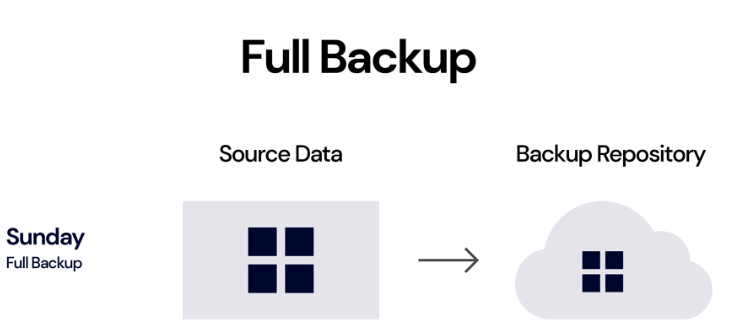
\includegraphics[width=0.5\textwidth]{img/fullb.png}  
    \caption{Representatie van een full back-up \autocite{Rivas2022}}   
    \label{fig:fullback-up}           
\end{figure}
Verschillende methoden en technologieën worden gebruikt om de veiligheid en betrouwbaarheid van data te garanderen. Een fundamentele back-upstrategie is de full back-up, waarbij de volledige inhoud van een bestandssysteem wordt gekopieerd naar een back-upapparaat \autocite{Beard2018}. Wanneer er zich een probleem voordoet, zoals het falen van een harde schijf, kan het hele bestandssysteem vanaf deze back-up volledig worden hersteld op een nieuwe schijf. Daarnaast kunnen ook individuele bestanden die verloren zijn gegaan, gemakkelijk worden teruggehaald uit de back-up. Dit soort back-up zorgt ervoor dat alle gegevens veilig zijn opgeslagen, maar heeft wel twee belangrijke nadelen. Ten eerste is het proces van het lezen en schrijven van het volledige bestandssysteem tijdsintensief, vooral bij grote hoeveelheden data. Ten tweede gebruikt het opslaan van een volledige kopie van het bestandssysteem veel opslagruimte, wat inefficiënt kan zijn wanneer de back-ups regelmatig worden gemaakt \autocite{Chervenak1998}.


\subsubsection{Incremental back-up}

Incremental back-ups zijn een efficiënte methode om alleen gewijzigde data sinds de laatste back-up op te slaan, wat tijd en opslag bespaart. In tegenstelling tot een volledige back-up, die alle data kopieert, richten incrementele back-ups zich enkel op nieuwe of aangepaste bestanden. Dit maakt ze sneller, maar hersteltijden kunnen langer zijn omdat meerdere incrementele back-ups nodig zijn naast de laatste volledige back-up. Recente onderzoeken hebben zich gericht op het optimaliseren van back-upstrategieën, met name voor databasesystemen. Zo zijn er modellen ontwikkeld die bepalen hoe vaak volledige en incrementele back-ups moeten worden uitgevoerd op basis van factoren zoals systeem-betrouwbaarheid, de hoeveelheid dataveranderingen en back-up-kosten \autocite{Zhao2024}. Er zijn ook varianten zoals differentiële back-ups, die alle veranderingen sinds de laatste volledige back-up bevatten, waardoor de hersteltijd korter kan zijn dan bij traditionele incrementele back-ups. Daarnaast zorgen moderne geautomatiseerde oplossingen voor continue incrementele back-ups, wat realtime herstelmogelijkheden biedt zonder noemenswaardige belasting van de productieomgeving \autocite{Qian2010}.
\begin{figure}[h] 
    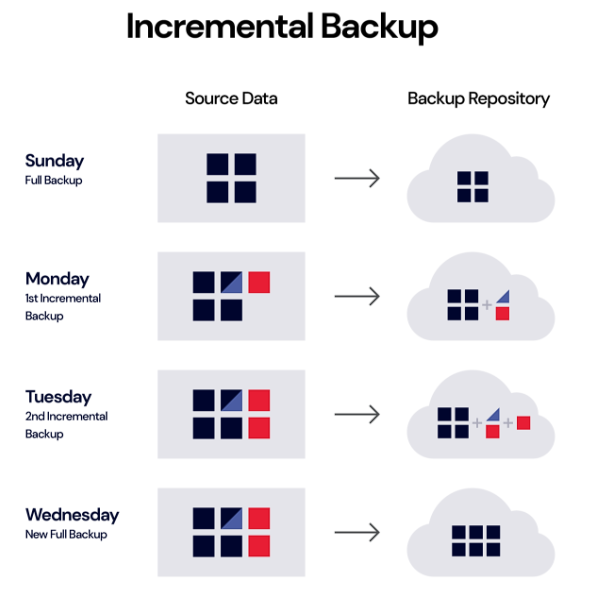
\includegraphics[width=0.5\textwidth]{img/incrementb.png}  
    \caption{Representatie van een incremental back-up \autocite{Rivas2022}}   
    \label{fig:incrback-up}           
\end{figure}


\subsubsection{Differentiële back-up}

Een differentiële back-up is een soort back-up waarbij alleen de data die sinds de laatste volledige back-up is veranderd of toegevoegd, wordt gekopieerd. In tegenstelling tot een incrementele back-up, die enkel de veranderingen sinds de laatste back-up opslaat, wordt er bij een differentiële back-up enkel de wijzigingen opgeslagen sinds de laatste full back-up . Dit komt doordat elke differentiële back-up alle wijzigingen sinds de meest recente volledige back-up bevat, waardoor de grootte van de back-up groter wordt naarmate er meer wijzigingen plaatsvinden. Een belangrijk voordeel van differentiële back-ups is de relatief snelle hersteltijd \autocite{Beard2018}. Om data te herstellen, is alleen de laatste volledige back-up en de meest recente differentiële back-up nodig, wat het herstelproces eenvoudiger en sneller maakt dan bij incrementele back-ups. Differentiële back-ups zijn bijzonder nuttig in omgevingen waar een snel herstelproces cruciaal is, zoals bij bedrijven die minimale downtime vereisen. Het nadeel van differentiële back-ups is dat de back-ups groter worden naargelang de tijd tussen de volledige back-ups. Elke nieuwe differentiële back-up bevat namelijk alle wijzigingen sinds de laatste volledige back-up, wat betekent dat deze geleidelijk groter wordt totdat er een nieuwe volledige back-up wordt gemaakt. Daarom is het belangrijk om een goede balans te vinden tussen de frequentie van volledige back-ups en differentiële back-ups.
 \begin{figure}[h]
     \centering
     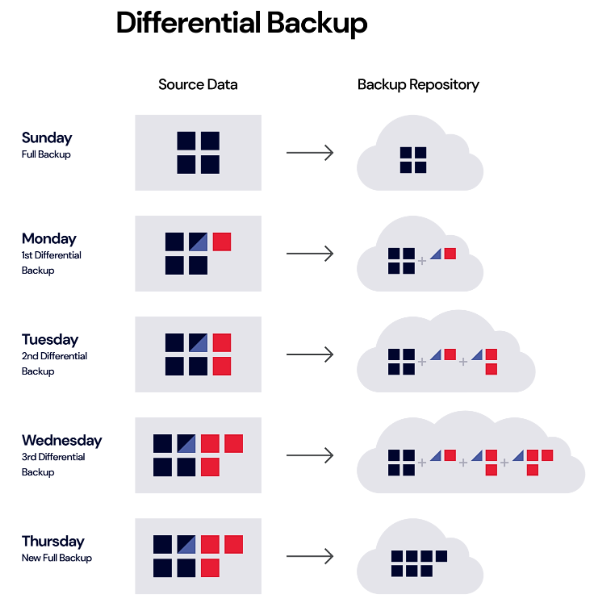
\includegraphics[width=0.5\textwidth]{img/diff.png}  
     \caption{Representatie van een differentiële back-up \autocite{Rivas2022}}   
     \label{fig:diffrback-up}           
 \end{figure}

\subsubsection{On-premise back-ups}
Bedrijven staan vaak voor de uitdaging om te beslissen of ze hun data on-premise opslaan of de voorkeur geven aan een cloud-service \autocite{Ali2024}. On-premise back-ups slaan gegevens lokaal op, meestal op fysieke schijven binnen het bedrijf zelf. Deze methode biedt bedrijven volledige controle over hun back-up- en gegevensbeheer. Een belangrijk voordeel van on-premise back-ups is dat data altijd beschikbaar is, zelfs zonder toegang tot het internet, wat nuttig is bij netwerkproblemen \autocite{Trovato2019}. Daarnaast hebben bedrijven volledige eigendom over de beveiliging van hun gegevens, aangezien de opslag lokaal blijft binnen het bedrijf. Hoewel deze methode geen terugkerende kosten aan externe providers met zich meebrengt, brengt het wel risico’s met zich mee, zoals schade door brand of overstromingen, en vraagt het om regelmatige onderhoud van de hardware. Het herstelproces is doorgaans sneller dan bij een cloudservice, wat van cruciaal belang kan zijn na een ransomware-aanval of een ander incident.
\subsubsection{Cloud-gebaseerde back-ups}
Cloud-gebaseerde back-ups zijn een populaire oplossing waarbij data extern wordt opgeslagen bij een bedrijf dat cloudservices aanbiedt. Dit biedt individuen en bedrijven de mogelijkheid om hun gegevens veilig op afstand te bewaren, zonder dat ze hoeven te investeren in fysieke opslagapparaten. Hoewel dit handig is om gegevensverlies te voorkomen bij hardware- of softwarestoringen, of onverwachte rampen, brengt het gebruik van cloud-opslag vaak aanzienlijke kosten met zich mee, vooral op de lange termijn \autocite{Obrutsky2016}. Naarmate je meer opslag nodig hebt is er altijd een mogelijkheid om te opschalen, dit is een groot voordeel van het gebruiken van een cloudservice. Echter, het waarborgen van de veiligheid van deze data is een cruciaal aandachtspunt, vooral omdat cloudproviders vaak niet open zijn over hoeveel kopieën van de data er zijn en waar deze precies worden opgeslagen. Om problemen zoals datalekken en foutieve verwijdering te voorkomen, zijn er nieuwe methoden zoals ``assured deletion'' ontwikkeld, waarmee klanten zeker weten dat hun gegevens permanent worden verwijderd op verzoek. Hierdoor kunnen bedrijven hun data met zekerheid beheren in de cloud terwijl gevoelige informatie veilig blijft \autocite{Rahumed2011}.


\subsubsection{Offline back-ups}
Offline back-ups zijn een traditionele methode waarbij data wordt opgeslagen op fysieke media, meestal externe harde schijven zonder tussenkomst van het internet. Het voornaamste voordeel is dat de data dan beveiligd is tegen online bedreigingen en er geen internettoegang nodig is om aan de data te geraken  \autocite{Edwards2022}. Een belangrijk voordeel is dat offline back-ups niet beïnvloed worden door stroomstoringen of internetuitval, waardoor ze een robuuste back-upoptie vormen voor gevoelige data. Echter, in tegenstelling tot on-premise back-ups, die vaak op dezelfde fysieke locatie als de IT-infrastructuur van een bedrijf worden opgeslagen, kunnen offline back-ups eenvoudig meegenomen en elders bewaard worden, waardoor ze extra bescherming bieden tegen fysieke rampen. Toch delen beide methoden het nadeel dat ze kwetsbaar zijn voor schade door ongelukken, diefstal of verlies, en moeten de fysieke apparaten op een veilige locatie opgeslagen worden \autocite{James2019}.

\subsubsection{Immutable storage}
Immutable storage is een type opslag waarbij data niet meer kan worden gewijzigd of aangepast vanaf het geback-upt is. Dit concept is cruciaal voor het waarborgen van de integriteit van belangrijke gegevens. Het idee achter immutability is dat bepaalde bestanden, nadat ze zijn gemaakt, niet meer mogen worden gewijzigd zonder de juiste autorisatie. Dit biedt een sterke bescherming tegen ongewenste wijzigingen en hierdoor kunnen hackers de gegevens niet aanpassen. Immutable storage speelt dus een belangrijke rol in het beschermen van systemen tegen cyberaanvallen. Bij aanvallen, waarbij hackers volledige toegang verkrijgen, kunnen onbeveiligde systemen worden gemanipuleerd of misbruikt. Immutable storage voorkomt dit, omdat de opgeslagen gegevens niet kunnen worden gewijzigd, zelfs niet door iemand met volledige toegang. Hierdoor wordt de integriteit van de data behouden en is het risico op schade door hackers aanzienlijk kleiner \autocite{Hasan2005}.

%---------- Methodologie ------------------------------------------------------
\section{Methodologie}%
\label{sec:methodologie}
In de eerste fase van het onderzoek zal er een grondige literatuurstudie worden uitgevoerd rond back-upstrategieën, ransomware-resistentie, en immutable storage met een overzicht van de state of the art van back-upstrategieën en immutabele opslag als deliverable. Wetenschappelijke papers, bedrijfscasussen en technische artikels zullen gebruikt worden om een theoretische basis aan te leggen en om de best-practices te achterhalen. Dit zal ook helpen om de onderzoeksvragen te beantwoorden. Daarnaast zal er een Proof-Of-Concept ontworpen worden waarbij onderzocht zal worden hoe er immutable back-ups gemaakt kunnen worden voor de back-ups van Forvis Mazars.  Daarnaast zal er een testomgeving opgezet worden om een ransomware-aanval na te bootsen en het systeem opnieuw op gang te krijgen. De deliverable voor de PoC is een werkende immutable back-upoplossing in Azure die tegen een ransomware-aanval bestendig is. Verder zal er een optimale back-upstrategie opgesteld worden met de state-of-the-art technieken. De literatuurstudie zal ongeveer 4 weken duren, de Proof-Of-Concept zal 4 weken duren en als laatst zal het rapport met de optimale verbeteringen 2 weken duren.

%---------- Verwachte resultaten ----------------------------------------------
\section{Verwacht resultaat, conclusie}%
\label{sec:verwachte_resultaten}
Het verwachte resultaat is dat door de implementatie van immutable storage en automatische back-ups, de back-upstrategie van Forvis Mazars zal worden verbeterd. Vooral de bescherming tegen ransomware en andere bedreigingen zal beter zijn door het gebruik van immutable storage, waarbij back-ups onveranderlijk worden opgeslagen en niet kunnen worden gemanipuleerd. Daarnaast zorgt de automatisering van de back-ups voor een efficiënter beheer, waarbij de manuele taken van het IT-team verminderd worden. Dit kan in de praktijk leiden tot meer consistente back-ups en een verbeterde betrouwbaarheid van het systeem. De resultaten zullen waarschijnlijk aantonen dat de combinatie van deze twee oplossingen zorgen voor een sterkere, efficiëntere en beter back-upstrategie.



%%---------- Andere bijlagen --------------------------------------------------
% TODO: Voeg hier eventuele andere bijlagen toe. Bv. als je deze BP voor de
% tweede keer indient, een overzicht van de verbeteringen t.o.v. het origineel.
%\input{...}

%%---------- Backmatter, referentielijst ---------------------------------------

\backmatter{}

\setlength\bibitemsep{2pt} %% Add Some space between the bibliograpy entries

\printbibliography[heading=bibintoc]
\end{document}
